\documentclass[a4paper]{article}
\usepackage[round]{natbib}
\bibliographystyle{abbrvnat}
\usepackage{pdfcolmk}
\usepackage{fancyvrb}
\usepackage{color}
\usepackage{url}
\usepackage[utf8]{inputenc}
%\VignetteIndexEntry{Tutorial} 
\usepackage{/home/stephane/Rdev/R-2.7.0/share/texmf/Sweave}
\begin{document}
\definecolor{Soutput}{rgb}{0,0,0.56}
\definecolor{Sinput}{rgb}{0.56,0,0}
\DefineVerbatimEnvironment{Sinput}{Verbatim}
{formatcom={\color{Sinput}},fontsize=\footnotesize, baselinestretch=0.75}
\DefineVerbatimEnvironment{Soutput}{Verbatim}
{formatcom={\color{Soutput}},fontsize=\footnotesize, baselinestretch=0.75}

\title{Moran's eigenvectors of spatial weighting matrices in 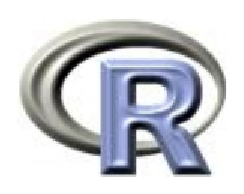
\includegraphics[width=1cm,keepaspectratio]{figs/Rlogo}}
\author{Stéphane Dray}
\maketitle


\begin{quote}
This appendix indicates how to manipulate spatial weighting matrices in R. It illustrates the approach developped in:
 Dray S., Legendre P. and Peres-Neto P. R. (accepted)
  Spatial modeling: a comprehensive framework for principal coordinate
  analysis of neighbor matrices (PCNM). \textit{Ecological Modelling}.
Commands are written in red and outputs are written in blue.
\end{quote} 
\tableofcontents
\section{Introduction}
R  is a statistical language which can be freely downloaded from internet (\url{http://www.r-project.org/}). The package \texttt{spdep} written by Roger Bivand is devoted to the creation and to the manipulation of spatial weighting matrices. You have to install it and to load it into your R session:
\begin{Schunk}
\begin{Sinput}
 library(spdep)
\end{Sinput}
\begin{Soutput}
Package 'spam' is loaded.  Version0.13-3 (2008-04-21).

Type demo( spam) for some demos,
 help( Spam) for an overview of this package.
\end{Soutput}
\end{Schunk}

\section{Spatial Neighborhood}
Spatial neighborhoods are managed in \texttt{spded} as objects of class \texttt{nb}. It corresponds to the notion of connectivity matrices discussed in the article. Various functions are devoted to create nb objects from geographic coordinates of sites. We present different alternatives according to the sampling plan.
\subsection{Grids}
If the sampling scheme is based on grid of 10 rows and 8 columns, you can easily generate the coordinates:

\begin{Schunk}
\begin{Sinput}
 xygrid <- expand.grid(1:10, 1:8)
 plot(xygrid)
\end{Sinput}
\end{Schunk}
\begin{center}
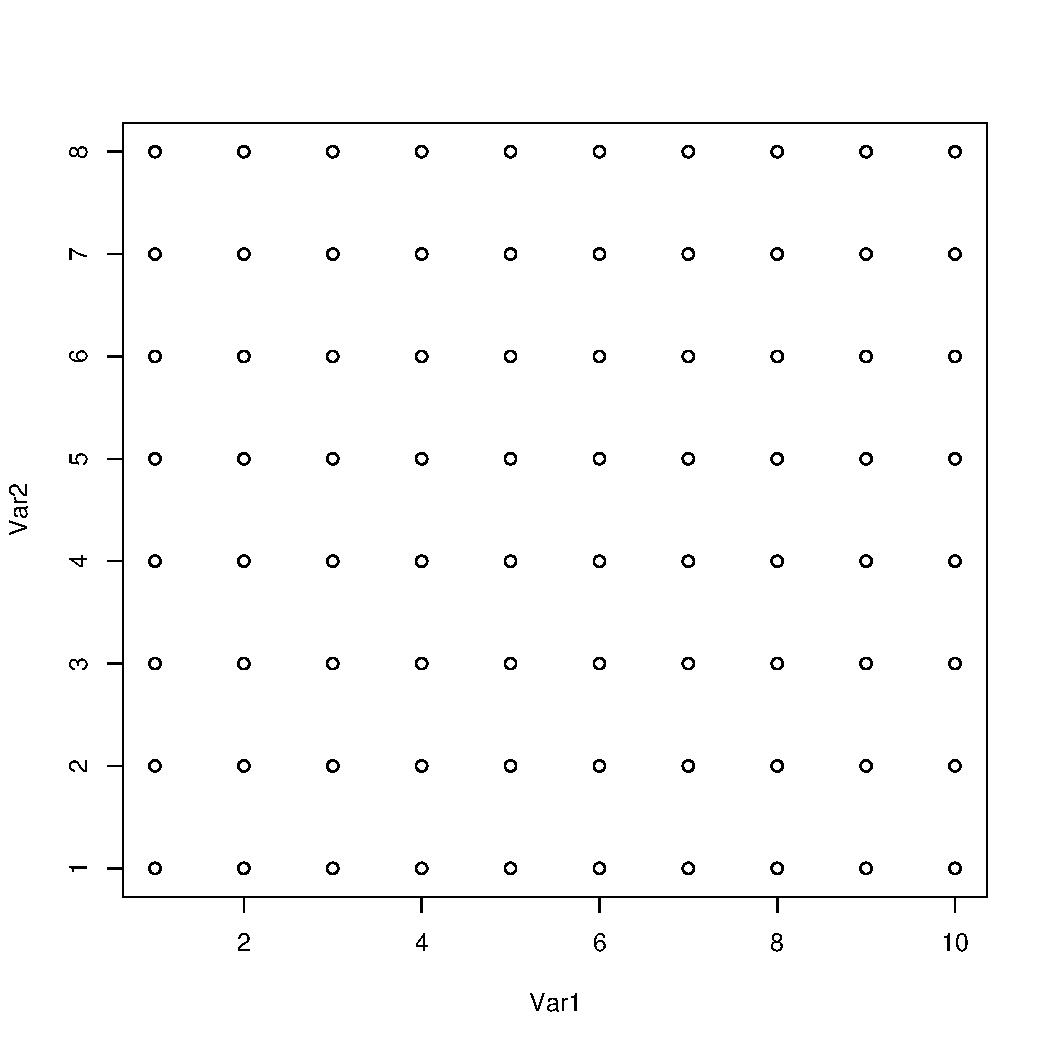
\includegraphics[width=0.8\textwidth,keepaspectratio]{figs/tutorial-ni2}
\end{center}

Spatial neighborhoods are managed in \texttt{spded} as objects of class \texttt{nb}. For a grid, you can create this kind of object with the function \texttt{cell2nb}.
\begin{Schunk}
\begin{Sinput}
 nb1 <- cell2nb(10, 8, type = "queen")
 plot(nb1, xygrid, col = "green", pch = 20, cex = 2)
 title(main = "queen neighborhood", cex.main = 2)
 nb1
\end{Sinput}
\begin{Soutput}
Neighbour list object:
Number of regions: 80 
Number of nonzero links: 536 
Percentage nonzero weights: 8.375 
Average number of links: 6.7 
\end{Soutput}
\end{Schunk}
\begin{Schunk}
\begin{Sinput}
 nb2 <- cell2nb(10, 8, type = "rook")
 plot(nb2, xygrid, col = "blue", pch = 20, cex = 2)
 title(main = "rook neighborhood", cex.main = 2)
 nb2
\end{Sinput}
\begin{Soutput}
Neighbour list object:
Number of regions: 80 
Number of nonzero links: 284 
Percentage nonzero weights: 4.438 
Average number of links: 3.55 
\end{Soutput}
\end{Schunk}

\begin{center}
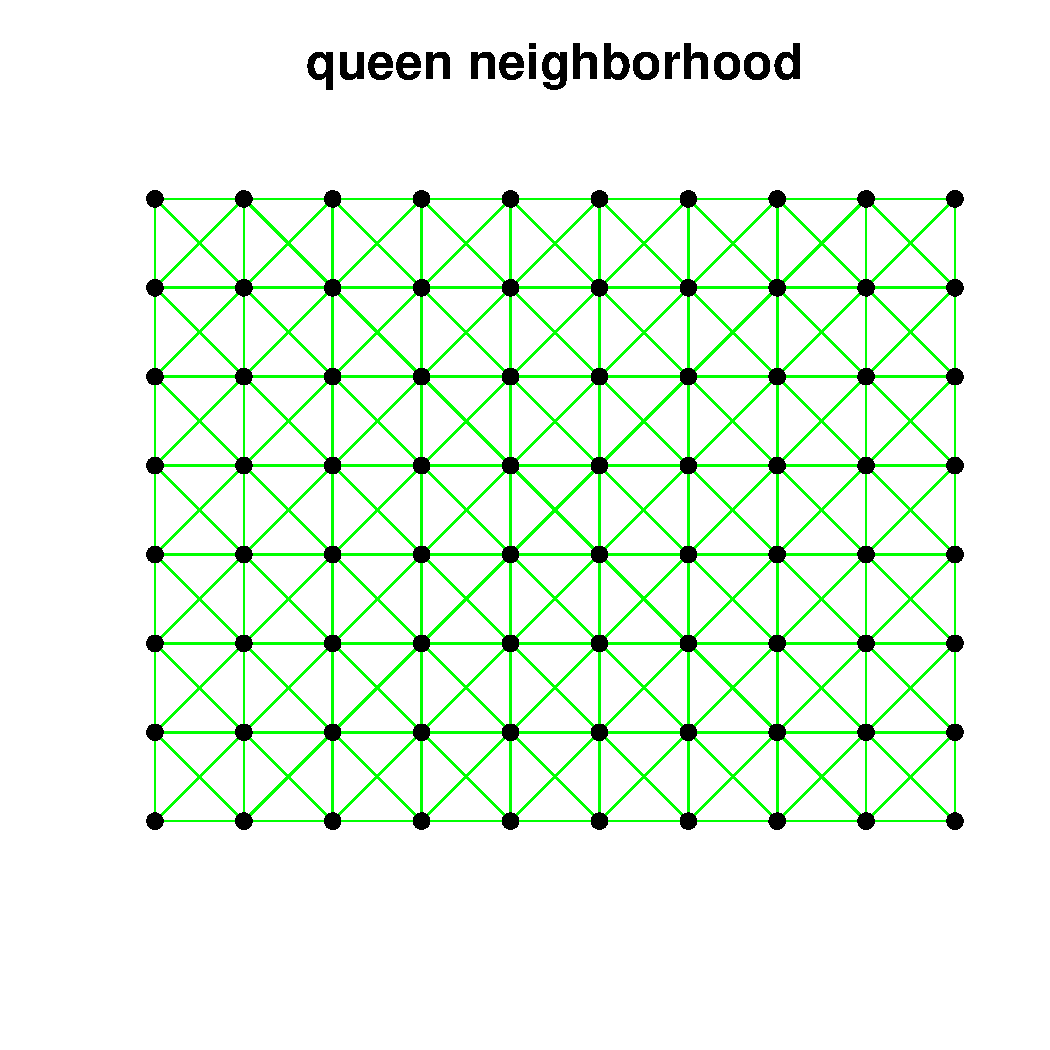
\includegraphics[width=0.4\textwidth,keepaspectratio]{figs/tutorial-ni3}
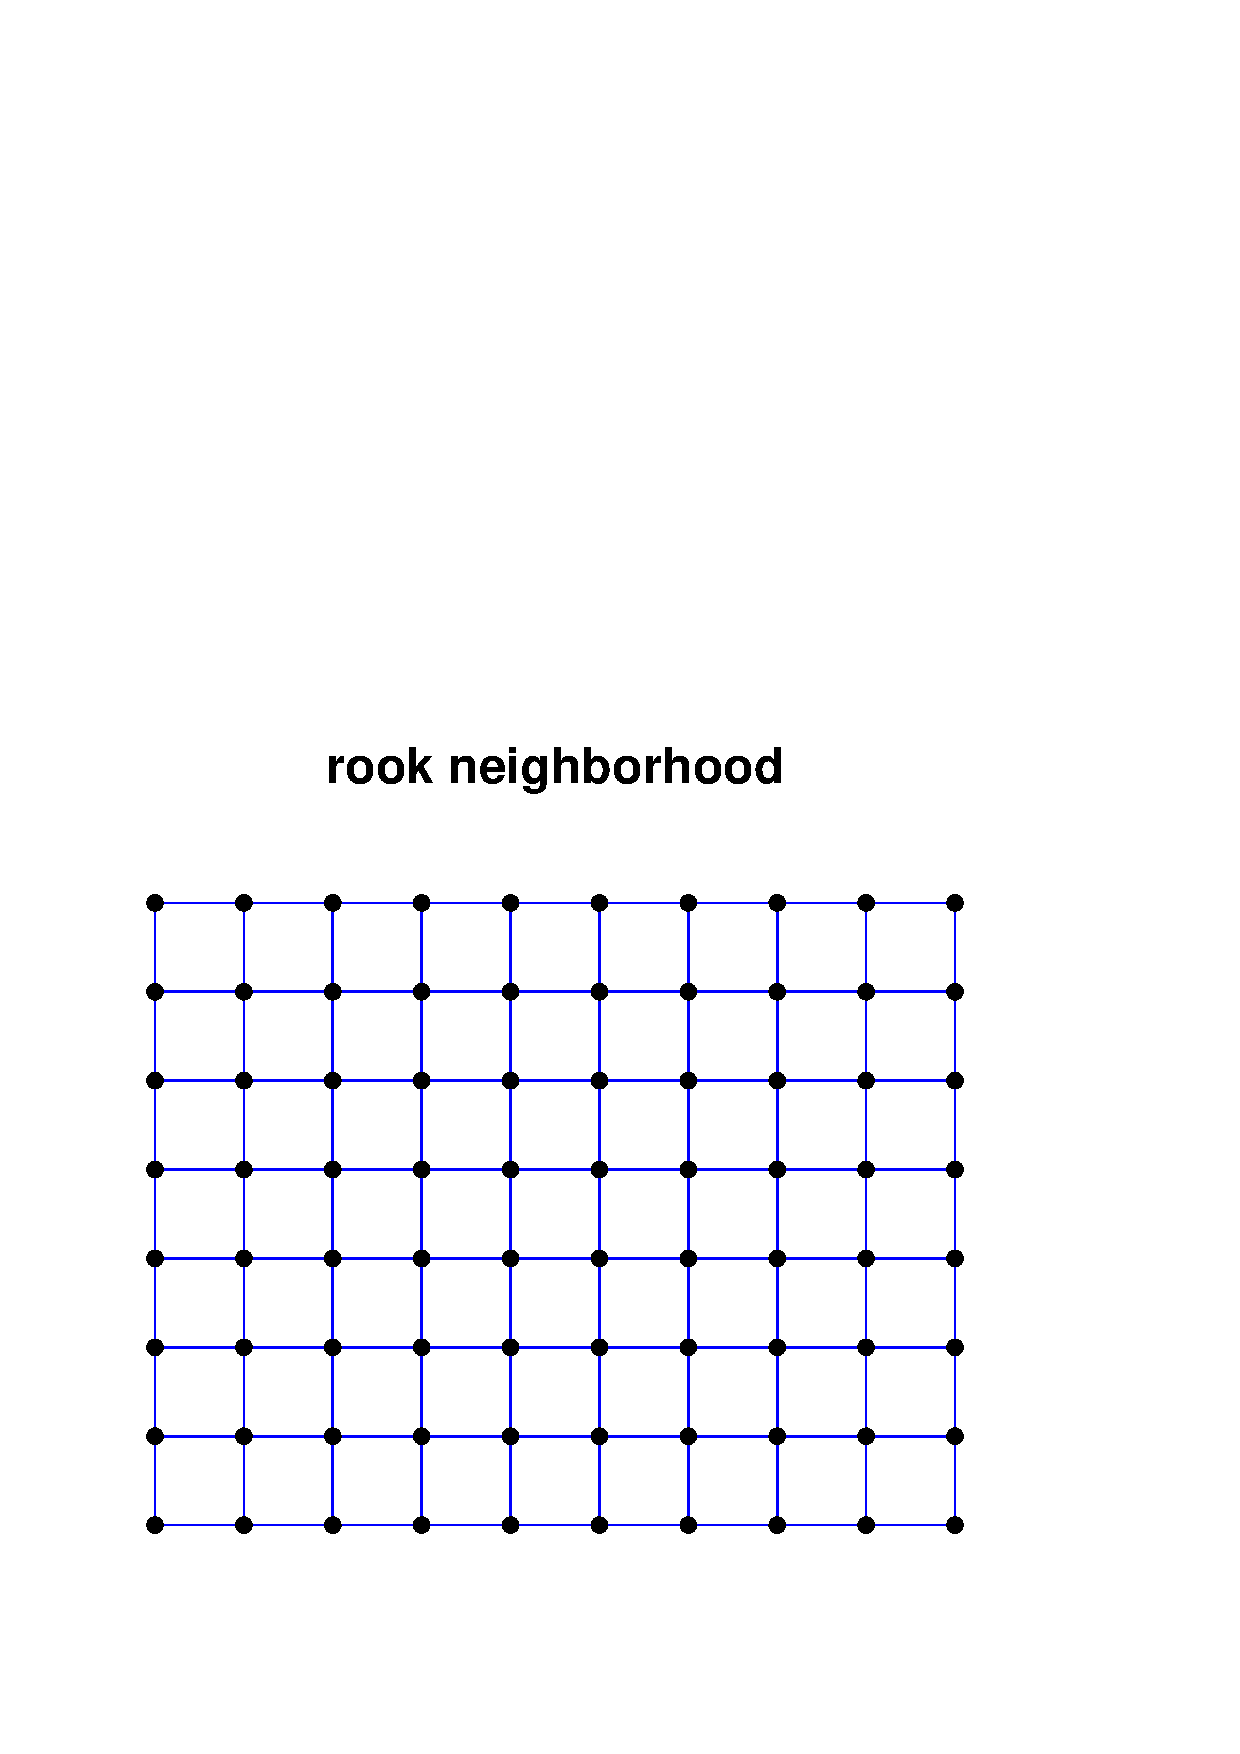
\includegraphics[width=0.4\textwidth,keepaspectratio]{figs/tutorial-ni4}
\end{center}
\subsection{Transects}
The easiest way to deal with transects is to consider them as grids with only one row:
\begin{Schunk}
\begin{Sinput}
 xytransect <- expand.grid(1:20, 1)
 nb3 = cell2nb(20, 1)
 plot(nb3, xytransect, col = "red", pch = 20, cex = 2)
 title(main = "transect of 20 sites")
 summary(nb3)
\end{Sinput}
\begin{Soutput}
Neighbour list object:
Number of regions: 20 
Number of nonzero links: 38 
Percentage nonzero weights: 9.5 
Average number of links: 1.9 
Link number distribution:

 1  2 
 2 18 
2 least connected regions:
1:1 20:1 with 1 link
18 most connected regions:
2:1 3:1 4:1 5:1 6:1 7:1 8:1 9:1 10:1 11:1 12:1 13:1 14:1 15:1 16:1 17:1 18:1 19:1 with 2 links
\end{Soutput}
\end{Schunk}
\begin{center}
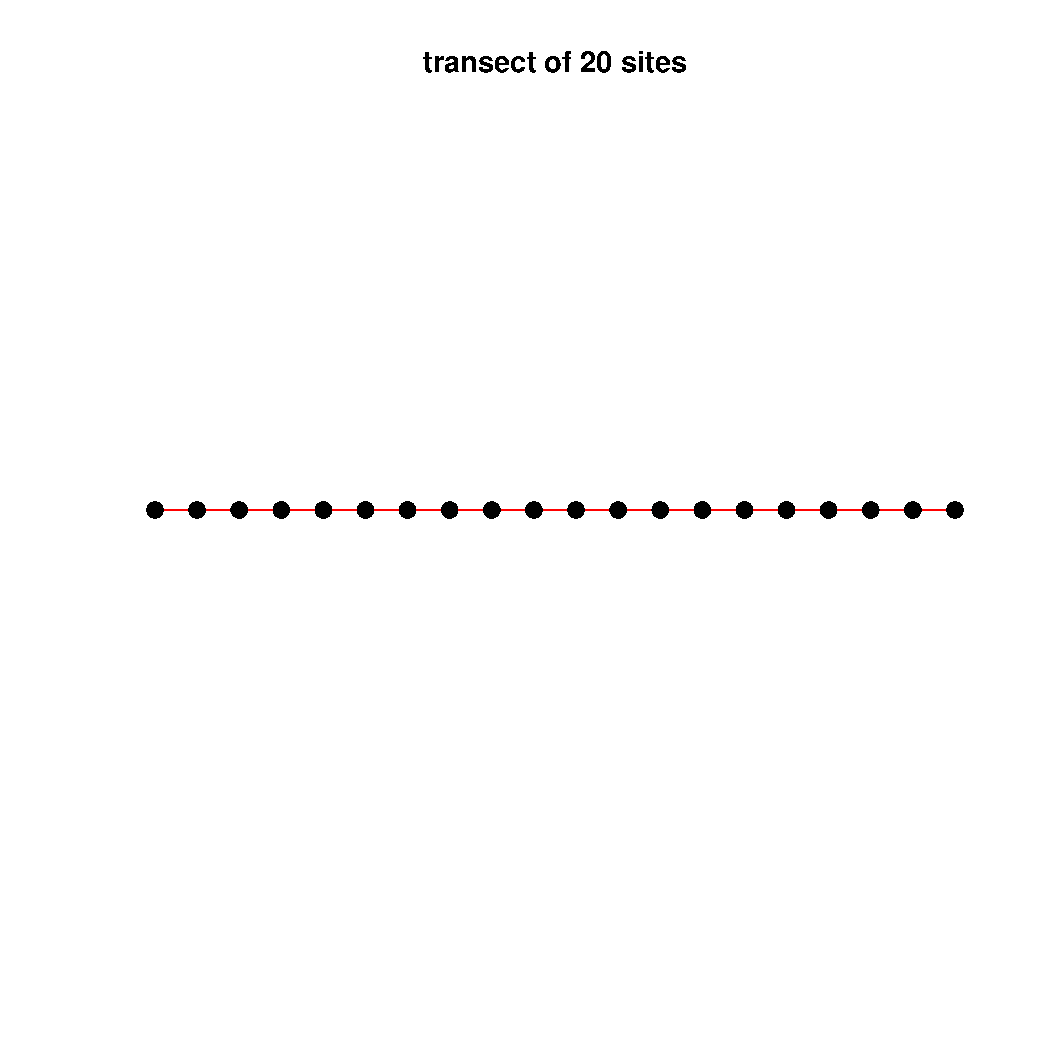
\includegraphics[width=0.6\textwidth,keepaspectratio]{figs/tutorial-ni5}
\end{center}
All sites have two neighbors except the first and the last one.
\subsection{Irregular samplings}
here are many ways to define neighborhood in the case of irregular samplings. We consider a sampling with 10 sites:
\begin{Schunk}
\begin{Sinput}
 set.seed(3)
 xyir <- matrix(runif(20), 10, 2)
 plot(xyir, pch = 20, cex = 1.5, main = "irregular sampling with 10 sites")
\end{Sinput}
\end{Schunk}
\begin{center}
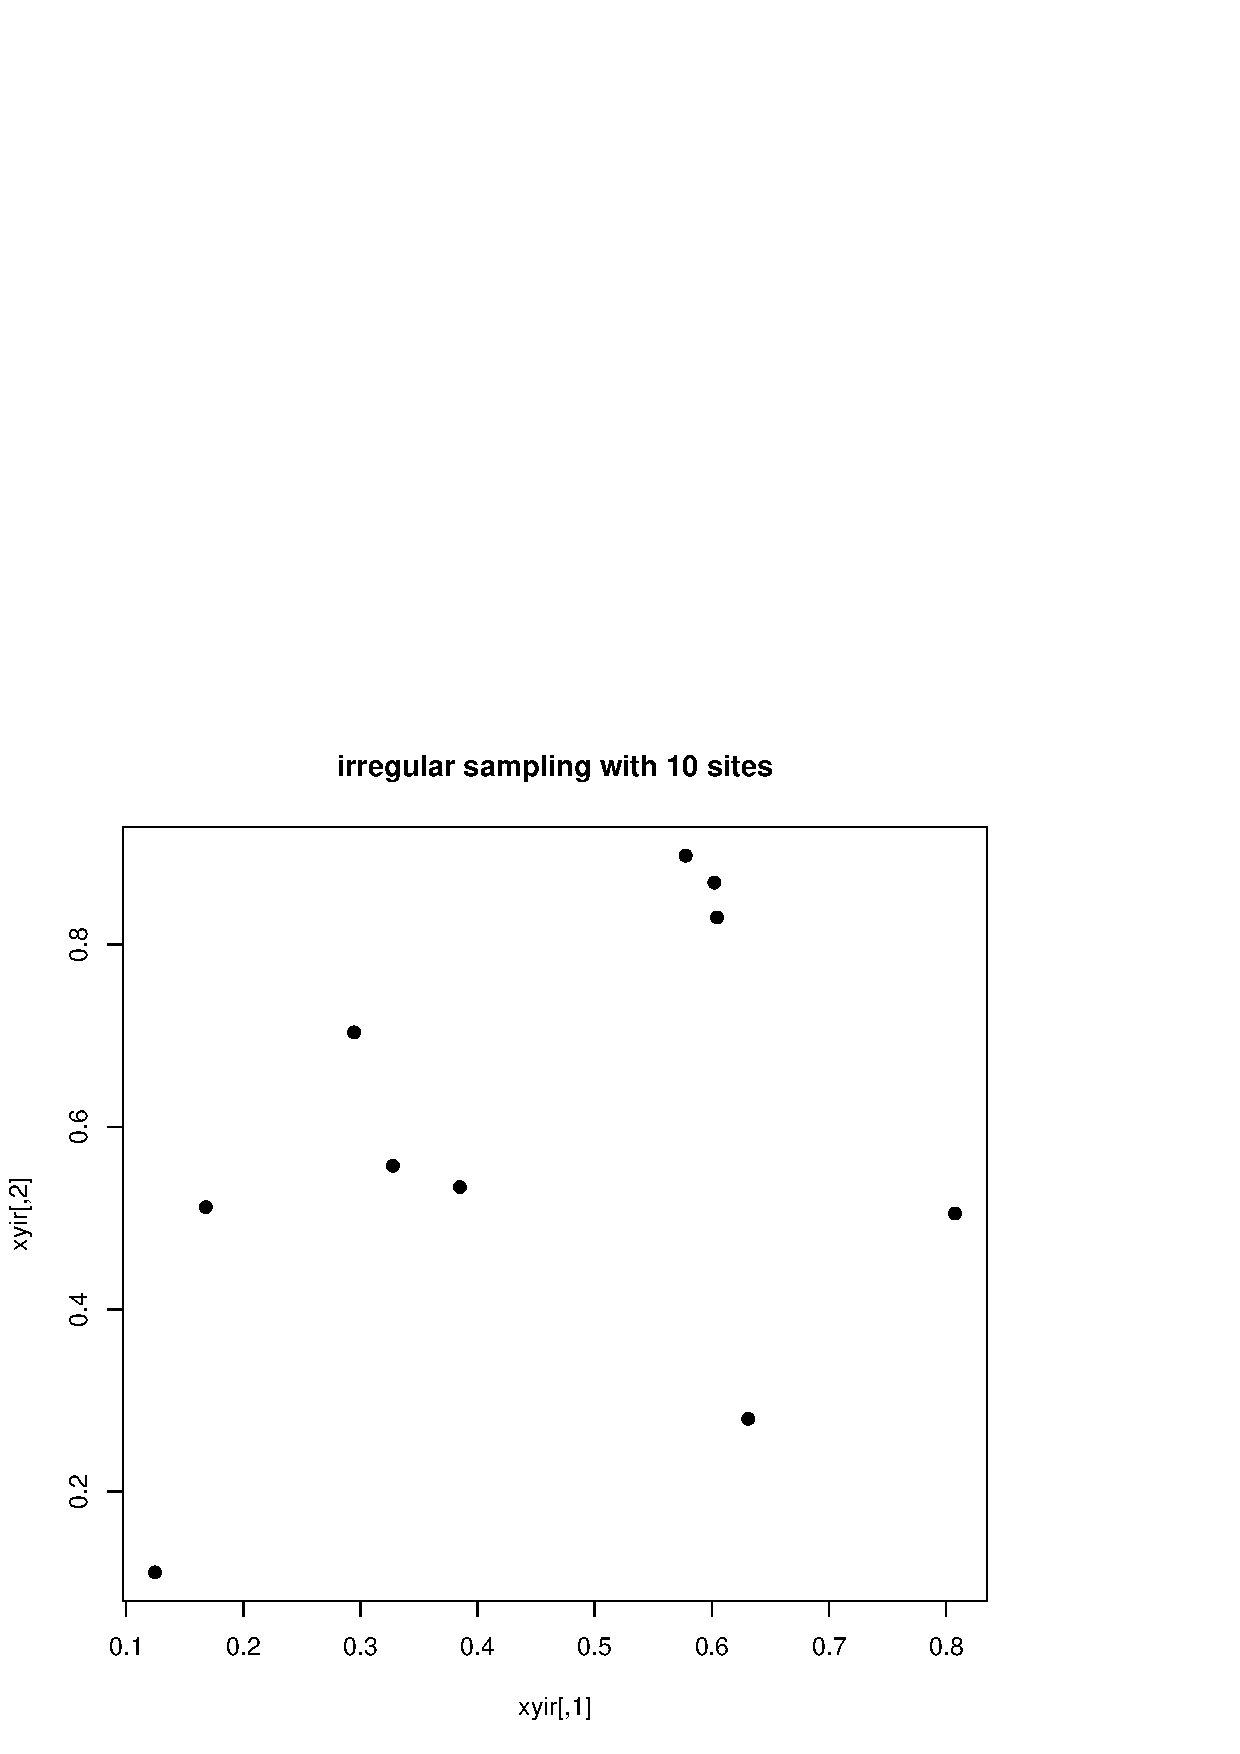
\includegraphics[width=0.6\textwidth,keepaspectratio]{figs/tutorial-ni6}
\end{center}
\begin{Schunk}
\begin{Sinput}
 nbnear1 <- dnearneigh(xyir, 0, 0.2)
 nbnear2 <- dnearneigh(xyir, 0, 0.3)
 nbnear3 <- dnearneigh(xyir, 0, 0.5)
 nbnear4 <- dnearneigh(xyir, 0, 1.5)
 par(mfrow = c(2, 2))
 plot(nbnear1, xyir, col = "red", pch = 20, cex = 2)
 title(main = "neighbors if 0<d<0.2")
 plot(nbnear2, xyir, col = "red", pch = 20, cex = 2)
 title(main = "neighbors if 0<d<0.3")
 plot(nbnear3, xyir, col = "red", pch = 20, cex = 2)
 title(main = "neighbors if 0<d<0.5")
 plot(nbnear4, xyir, col = "red", pch = 20, cex = 2)
 title(main = "neighbors if 0<d<1.5")
\end{Sinput}
\end{Schunk}
\begin{center}
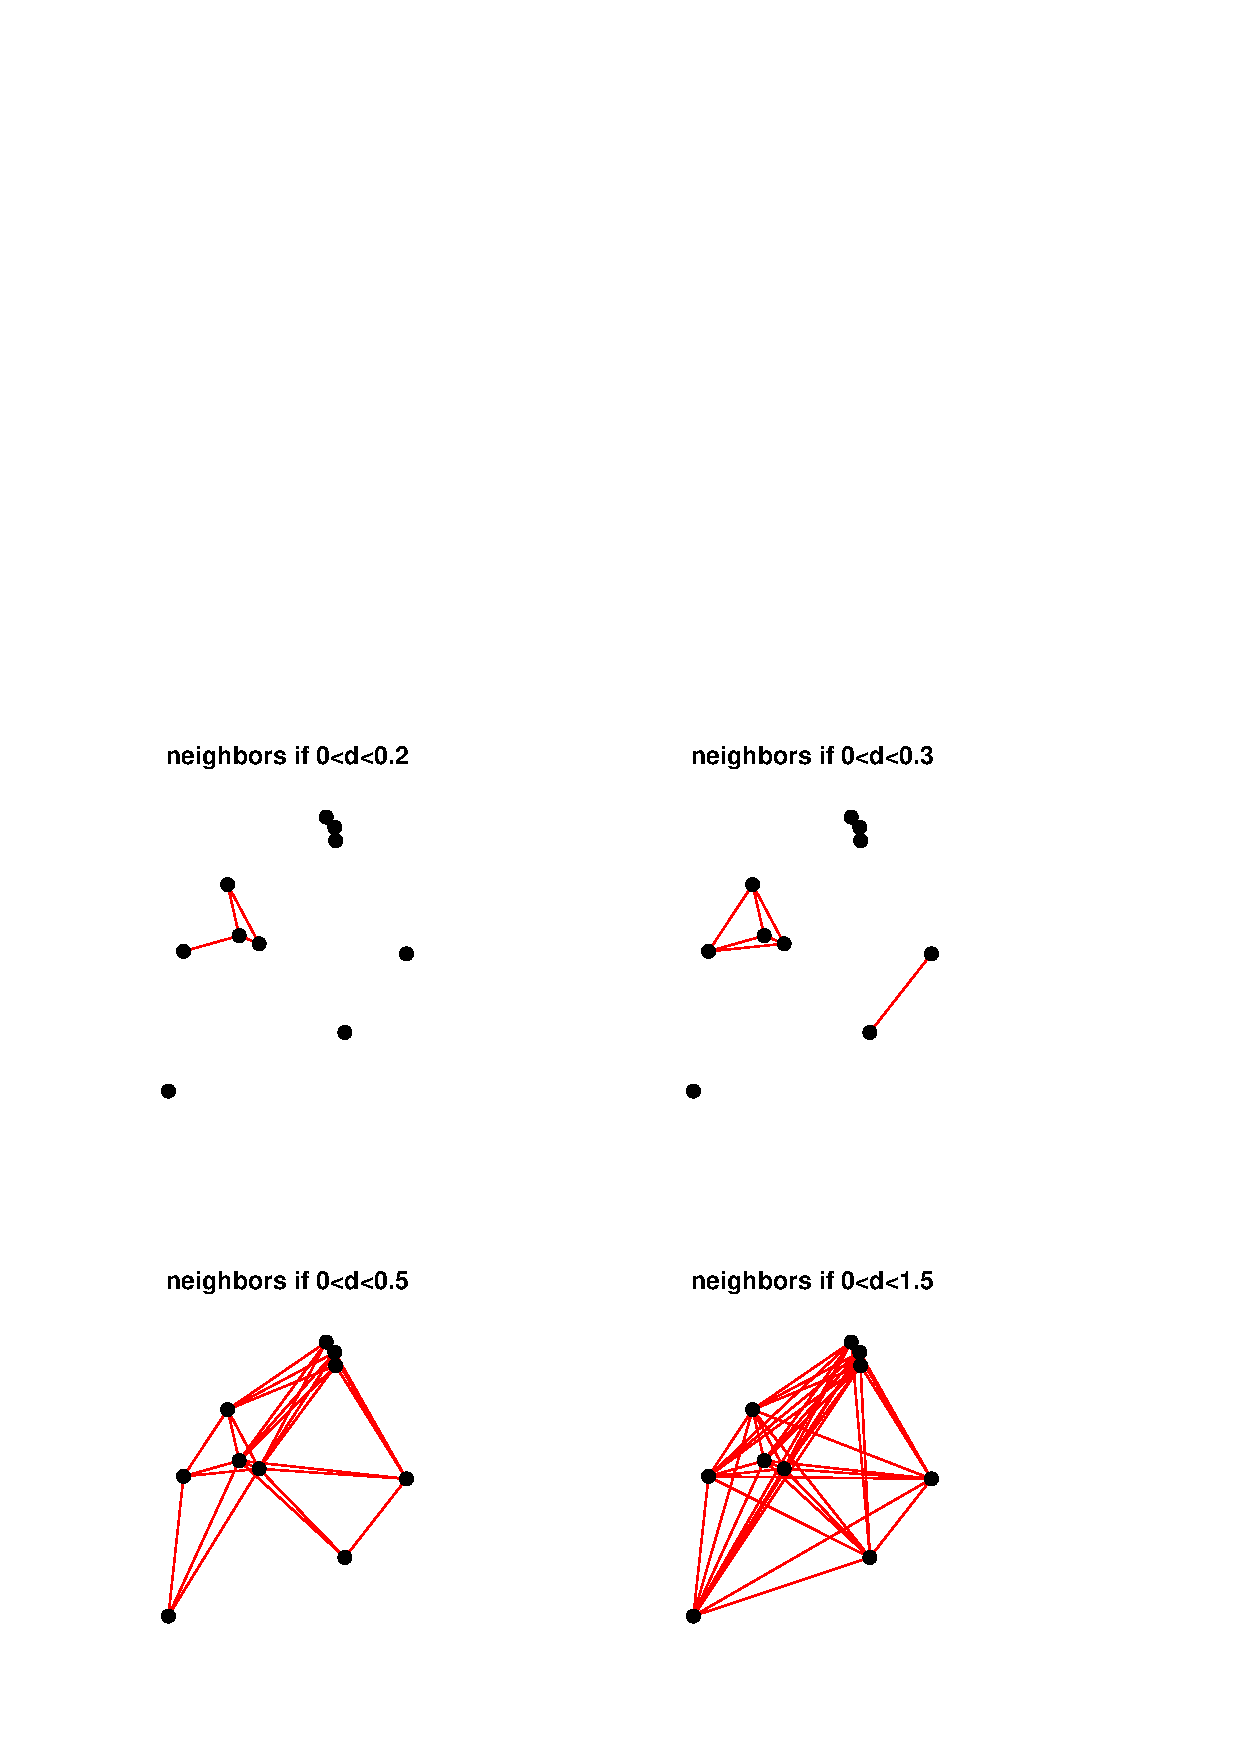
\includegraphics[width=0.8\textwidth,keepaspectratio]{figs/tutorial-ni7}
\end{center}
\begin{Schunk}
\begin{Sinput}
 nbnear1
\end{Sinput}
\begin{Soutput}
Neighbour list object:
Number of regions: 10 
Number of nonzero links: 14 
Percentage nonzero weights: 14 
Average number of links: 1.4 
3 regions with no links:
2 7 10
\end{Soutput}
\begin{Sinput}
 nbnear2
\end{Sinput}
\begin{Soutput}
Neighbour list object:
Number of regions: 10 
Number of nonzero links: 20 
Percentage nonzero weights: 20 
Average number of links: 2 
1 region with no links:
7
\end{Soutput}
\end{Schunk}
Note that some points have no neighbors.
\begin{Schunk}
\begin{Sinput}
 nbnear3
\end{Sinput}
\begin{Soutput}
Neighbour list object:
Number of regions: 10 
Number of nonzero links: 58 
Percentage nonzero weights: 58 
Average number of links: 5.8 
\end{Soutput}
\begin{Sinput}
 nbnear4
\end{Sinput}
\begin{Soutput}
Neighbour list object:
Number of regions: 10 
Number of nonzero links: 90 
Percentage nonzero weights: 90 
Average number of links: 9 
\end{Soutput}
\end{Schunk}
In the last case, all points are connected to the 9 others.

It is also possible to possible to define neighborhood by a criteria based on nearest neighbors. However, note that this option can lead to non-symmetric neighborhood: if site A is the nearest neighbor of site B, it does not mean that site B is the nearest neighbor of site A.

The function knearneigh creates an object of class \texttt{knn}. It can be transform into a \texttt{nb} object with the function \texttt{knn2nb}. Note that this function has a argument \texttt{sym} which can be set to \texttt{TRUE} if we want to force the output neighborhood to symmetry.
\begin{Schunk}
\begin{Sinput}
 knn1 <- knearneigh(xyir, k = 1)
 nbknn1 <- knn2nb(knn1, sym = T)
 plot(nbknn1, xyir, col = "red", pch = 20, cex = 2)
 title(main = "nearest neighbors (k=1)", cex.main = 2)
\end{Sinput}
\end{Schunk}
\begin{Schunk}
\begin{Sinput}
 knn2 <- knearneigh(xyir, k = 2)
 nbknn2 <- knn2nb(knn2, sym = T)
 plot(nbknn2, xyir, col = "red", pch = 20, cex = 2)
 title(main = "nearest neighbors (k=2)", cex.main = 2)
\end{Sinput}
\end{Schunk}

\begin{center}
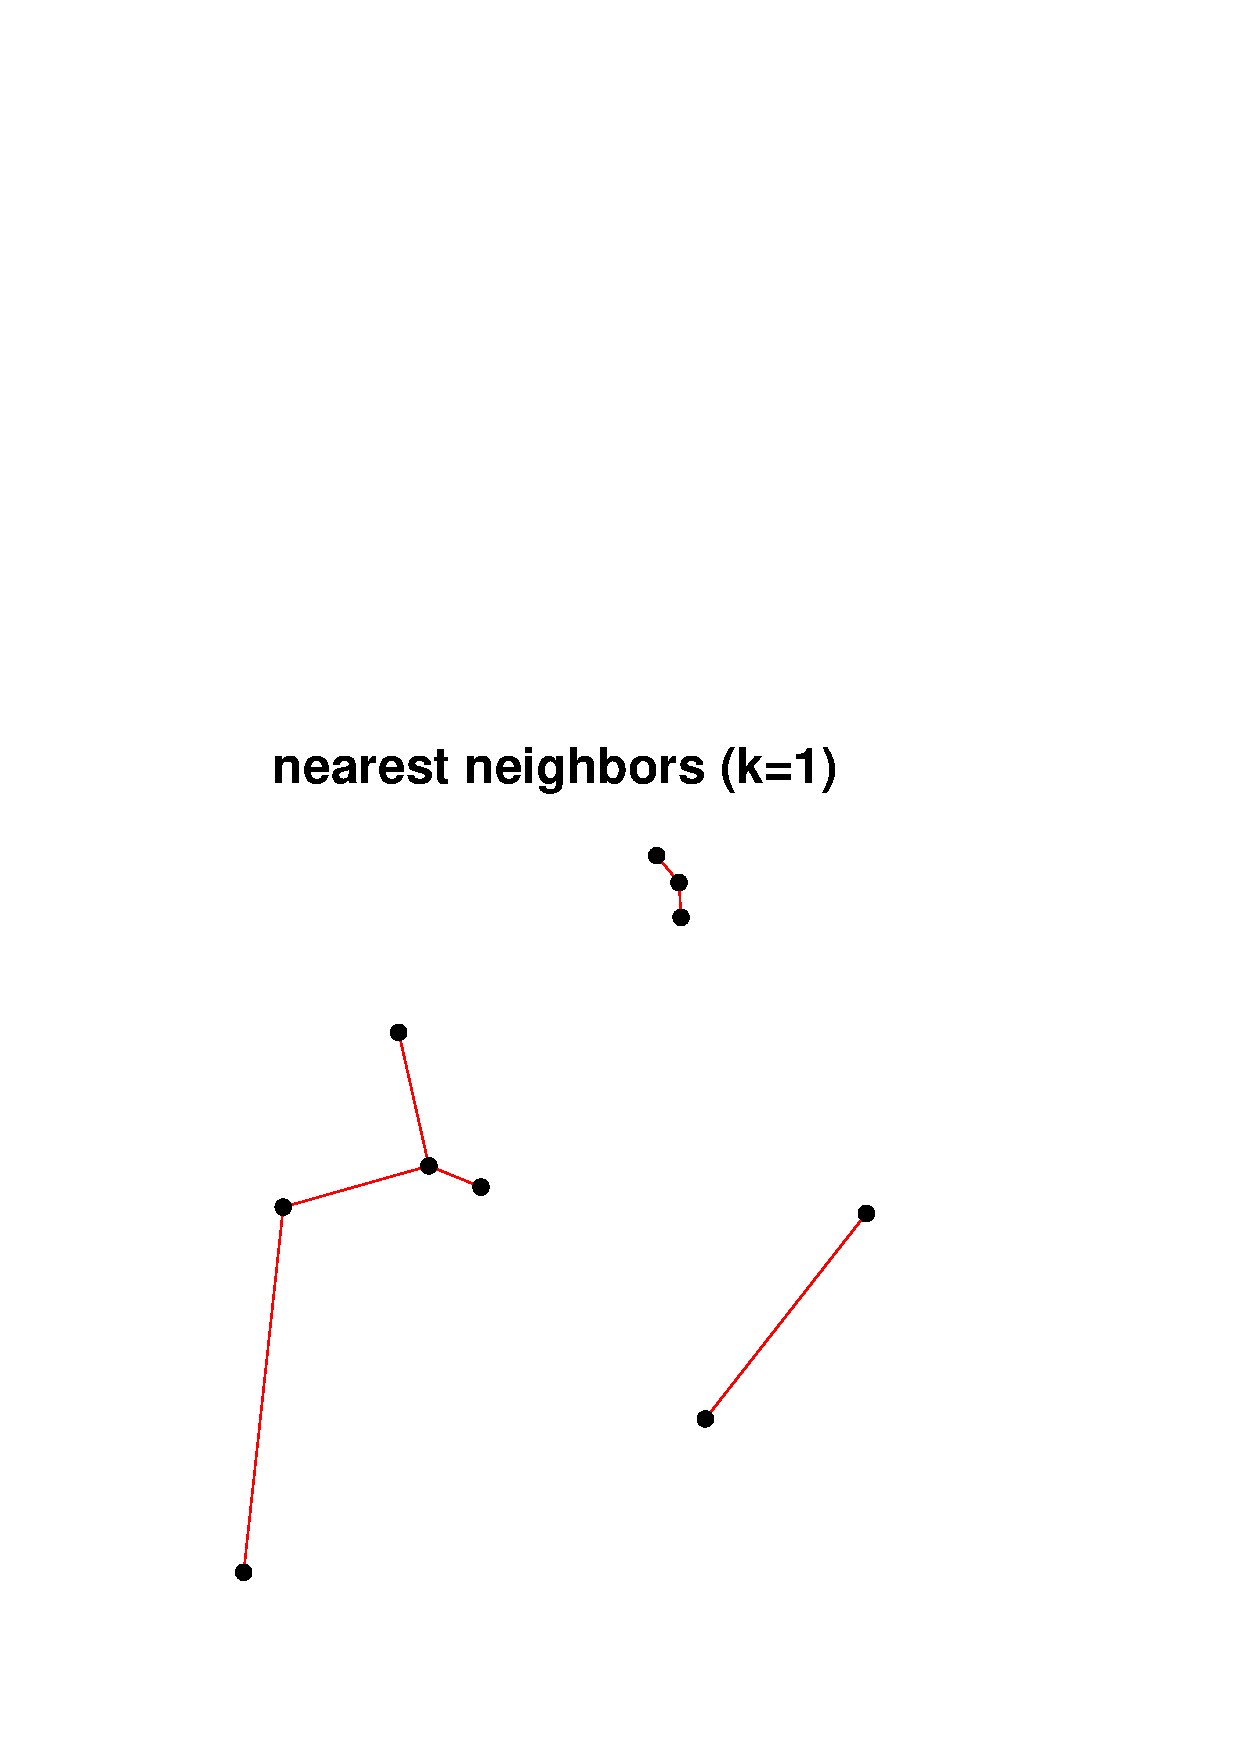
\includegraphics[width=0.4\textwidth,keepaspectratio]{figs/tutorial-ni10}
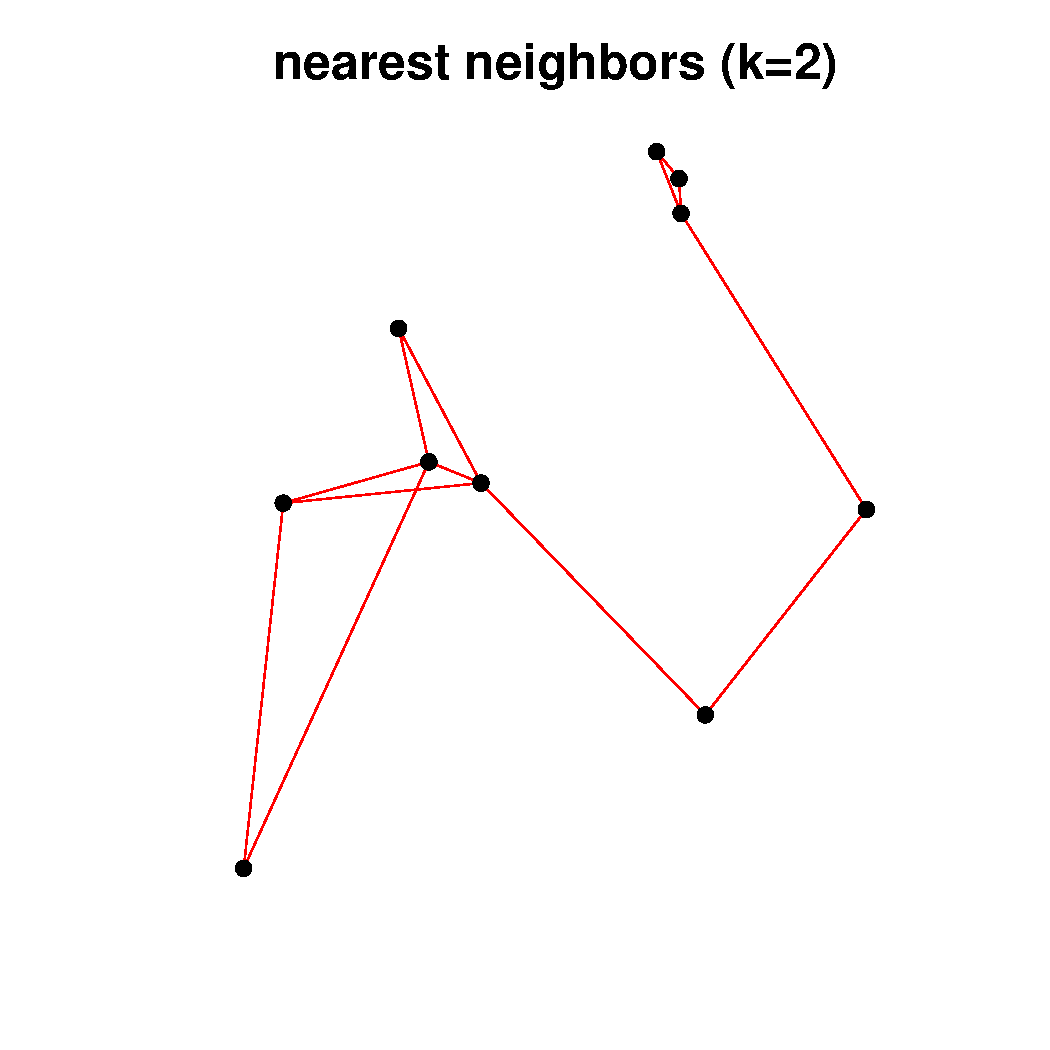
\includegraphics[width=0.4\textwidth,keepaspectratio]{figs/tutorial-ni11}
\end{center}

This definition of neighborhood can lead to unconnected subgraphs. The function \texttt{n.comp.nb} finds the number of disjoint connected subgraphs:
\begin{Schunk}
\begin{Sinput}
 n.comp.nb(nbknn1)
\end{Sinput}
\begin{Soutput}
$nc
[1] 3

$comp.id
 [1] 1 2 1 1 3 3 1 1 3 2
\end{Soutput}
\begin{Sinput}
 n.comp.nb(nbknn2)
\end{Sinput}
\begin{Soutput}
$nc
[1] 1

$comp.id
 [1] 1 1 1 1 1 1 1 1 1 1
\end{Soutput}
\end{Schunk}

More elaborate procedures are available to define neighborhood. For instance, Delaunay triangulation is obtained with the function \texttt{tri2nb}. It requires the package \texttt{tripack}. Other procedures are available (Gabriel graph, relative neighborhood...):
\begin{Schunk}
\begin{Sinput}
 nbtri <- tri2nb(xyir)
 nbgab <- graph2nb(gabrielneigh(xyir), sym = TRUE)
 nbrel <- graph2nb(relativeneigh(xyir), sym = TRUE)
 nbsoi <- graph2nb(soi.graph(nbtri, xyir), sym = TRUE)
 par(mfrow = c(2, 2))
 plot(nbtri, xyir, col = "red", pch = 20, cex = 2)
 title(main = "Delaunay triangulation")
 plot(nbgab, xyir, col = "red", pch = 20, cex = 2)
 title(main = "Gabriel Graph")
 plot(nbrel, xyir, col = "red", pch = 20, cex = 2)
 title(main = "Relative Neighbor Graph")
 plot(nbsoi, xyir, col = "red", pch = 20, cex = 2)
 title(main = " Sphere of Influence Graph")
\end{Sinput}
\end{Schunk}

\begin{center}
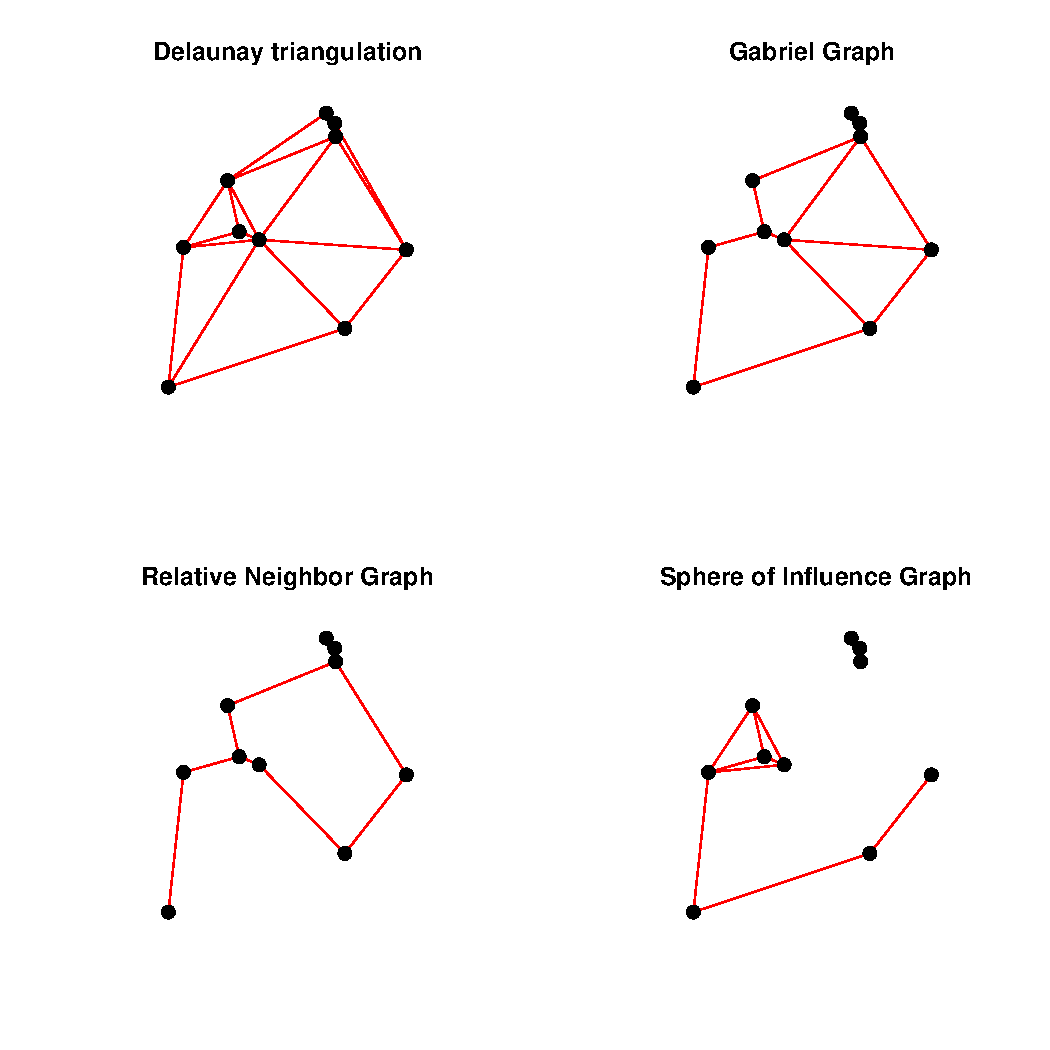
\includegraphics[width=0.8\textwidth,keepaspectratio]{figs/tutorial-ni13}
\end{center}

What are the differences between two neighborhoods ?
\begin{Schunk}
\begin{Sinput}
 diffnb(nbsoi, nbrel)
\end{Sinput}
\begin{Soutput}
Neighbour difference for region id: 1 in relation to id: 3 8 
Neighbour difference for region id: 2 in relation to id: 6 
Neighbour difference for region id: 3 in relation to id: 1 8 10 
Neighbour difference for region id: 6 in relation to id: 2 8 9 
Neighbour difference for region id: 7 in relation to id: 10 
Neighbour difference for region id: 8 in relation to id: 1 3 6 
Neighbour difference for region id: 9 in relation to id: 6 
Neighbour difference for region id: 10 in relation to id: 3 7 
Neighbour list object:
Number of regions: 10 
Number of nonzero links: 16 
Percentage nonzero weights: 16 
Average number of links: 1.6 
2 regions with no links:
4 5
\end{Soutput}
\end{Schunk}

Usually, it can be useful to remove some connections due to edge effects. If you want to modify the neighborhood, the function \texttt{edit.nb} provides an interactive tool to add or delete connections.
Lastly, we mention the function include.self to include the site itself in its own list of neighbors:
\begin{Schunk}
\begin{Sinput}
 str(nbsoi)
\end{Sinput}
\begin{Soutput}
List of 10
 $ : int [1:4] 3 4 7 8
 $ : int 10
 $ : int [1:3] 1 4 8
 $ : int [1:3] 1 3 8
 $ : int [1:2] 6 9
 $ : int [1:2] 5 9
 $ : int [1:2] 1 10
 $ : int [1:3] 1 3 4
 $ : int [1:2] 5 6
 $ : int [1:2] 2 7
 - attr(*, "region.id")= chr [1:10] "1" "2" "3" "4" ...
 - attr(*, "call")= language soi.graph(tri.nb = nbtri, coords = xyir)
 - attr(*, "class")= chr "nb"
 - attr(*, "sym")= logi TRUE
\end{Soutput}
\begin{Sinput}
 str(include.self(nbsoi))
\end{Sinput}
\begin{Soutput}
List of 10
 $ : int [1:5] 1 3 4 7 8
 $ : int [1:2] 2 10
 $ : int [1:4] 1 3 4 8
 $ : int [1:4] 1 3 4 8
 $ : int [1:3] 5 6 9
 $ : int [1:3] 5 6 9
 $ : int [1:3] 1 7 10
 $ : int [1:4] 1 3 4 8
 $ : int [1:3] 5 6 9
 $ : int [1:3] 2 7 10
 - attr(*, "region.id")= chr [1:10] "1" "2" "3" "4" ...
 - attr(*, "call")= language soi.graph(tri.nb = nbtri, coords = xyir)
 - attr(*, "class")= chr "nb"
 - attr(*, "sym")= logi TRUE
 - attr(*, "self.included")= logi TRUE
\end{Soutput}
\end{Schunk}
See also these functions for the manipulation of \texttt{nb} objects:
\begin{Sinput}
intersect.nb(nb.obj1,nb.obj2)
union.nb(nb.obj1,nb.obj2)
setdiff.nb(nb.obj1,nb.obj2)
complement.nb(nb.obj)

droplinks(nb, drop, sym=TRUE)

nblag(neighbours, maxlag)
\end{Sinput}
\subsection{Surface data}
If the sampling sites are polygons (and not points), you can use the function \texttt{poly2nb}. Note also that GIS data can be import into R using the package \texttt{shapefiles}. Then, utilities for transform/manipulate these data are available in the package \texttt{maptools}.
\begin{Schunk}
\begin{Sinput}
 library(maptools)
 data(columbus)
 xx <- poly2nb(polys)
 plot(polys, border = "grey")
 plot(xx, coords, add = TRUE, pch = 20, cex = 2, col = "red")
 title(main = "Neighborhood for polygons")
\end{Sinput}
\end{Schunk}
\begin{center}
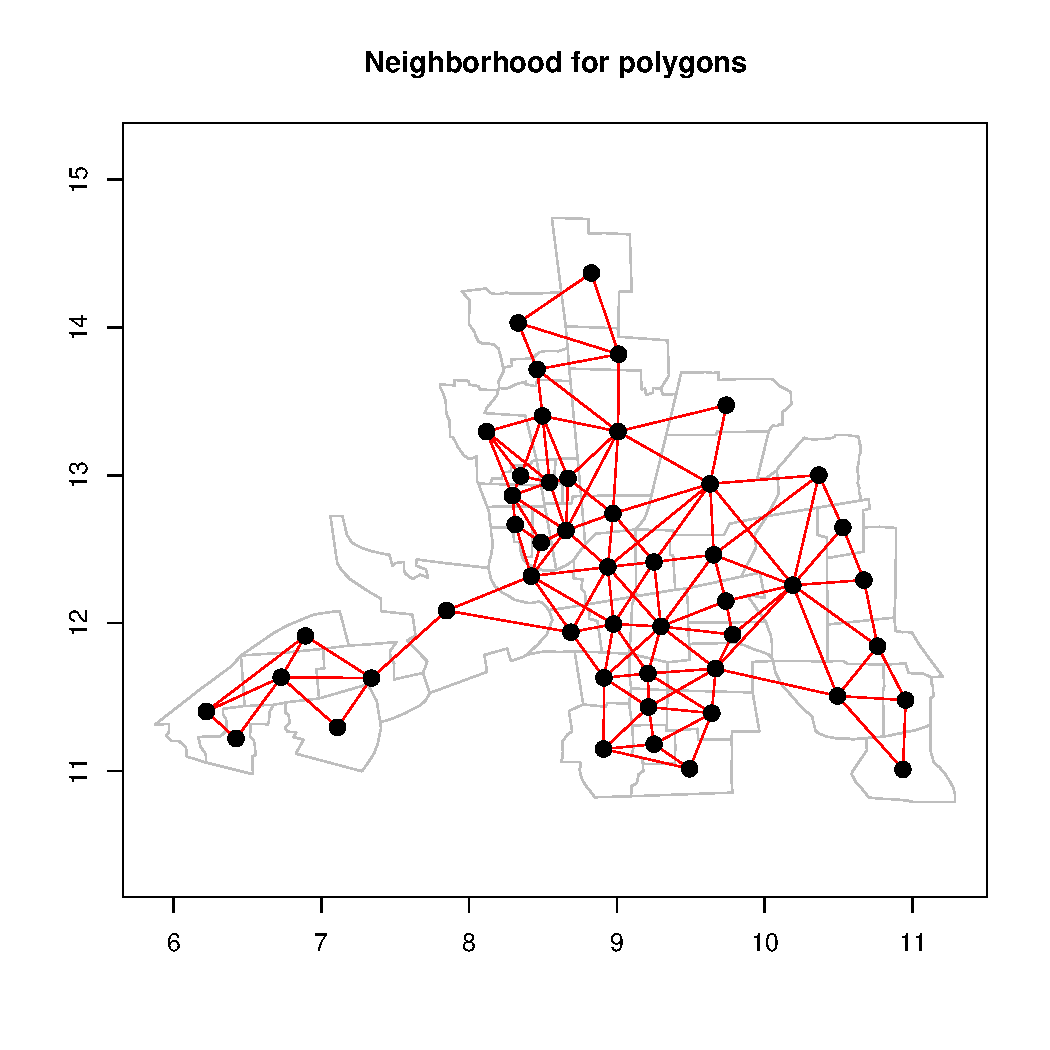
\includegraphics[width=0.8\textwidth,keepaspectratio]{figs/tutorial-ni16}
\end{center}
\section{Spatial weighting matrices}
Spatial weighting matrices are not stored as matrices but as objects of the class \texttt{listw}. This format is more efficient than a matrix representation to manage large data sets. You can easily create an object of class \texttt{listw} from an object of class \texttt{nb} with the function \texttt{nb2listw}.
Different objects \texttt{listw} can be obtained from a \texttt{nb} object. The argument \texttt{style} allow to define a transformation of the matrix such as standardization by row sum, by total sum or binary coding... General spatial weights can be introduced by the argument \texttt{glist}. This allows to introduce, for instance, a weighting relative to the distances between the points. For this task, the function \texttt{nbdists} could be very useful as it computes Euclidean distance between neighbor sites defined by an \texttt{nb} object.

A \texttt{nb} object is a list of neighbors. The neighbors of the first site:
\begin{Schunk}
\begin{Sinput}
 nbgab[[1]]
\end{Sinput}
\begin{Soutput}
[1] 4 7
\end{Soutput}
\end{Schunk}
We can compute Euclidean distance between sites and select distances for neighbors:
\begin{Schunk}
\begin{Sinput}
 round(dist(xyir), 3)
\end{Sinput}
\begin{Soutput}
       1     2     3     4     5     6     7     8     9
2  0.640                                                
3  0.218 0.424                                          
4  0.166 0.483 0.062                                    
5  0.561 0.417 0.398 0.414                              
6  0.540 0.383 0.368 0.388 0.038                        
7  0.403 0.788 0.496 0.490 0.895 0.864                  
8  0.230 0.550 0.192 0.150 0.349 0.334 0.616            
9  0.562 0.455 0.411 0.422 0.038 0.073 0.907 0.343      
10 0.518 0.286 0.354 0.411 0.589 0.551 0.534 0.541 0.620
\end{Soutput}
\end{Schunk}
It is done automatically by the function \texttt{nbdists}:
\begin{Schunk}
\begin{Sinput}
 distgab <- nbdists(nbgab, xyir)
 str(distgab)
\end{Sinput}
\begin{Soutput}
List of 10
 $ : num [1:2] 0.166 0.403
 $ : num [1:3] 0.424 0.383 0.286
 $ : num [1:4] 0.4236 0.0617 0.3682 0.3538
 $ : num [1:3] 0.1660 0.0617 0.1501
 $ : num [1:2] 0.0383 0.0384
 $ : num [1:4] 0.3830 0.3682 0.0383 0.3344
 $ : num [1:2] 0.403 0.534
 $ : num [1:2] 0.150 0.334
 $ : num 0.0384
 $ : num [1:3] 0.286 0.354 0.534
 - attr(*, "class")= chr "nbdist"
 - attr(*, "call")= language nbdists(nb = nbgab, coords = xyir)
\end{Soutput}
\end{Schunk}
Then, we can define weights as a function of distance (e.g. $1-d_{ij}/max(d_{ij})$):
\begin{Schunk}
\begin{Sinput}
 fdist <- lapply(distgab, function(x) 1 - x/max(dist(xyir)))
\end{Sinput}
\end{Schunk}
And the spatial weighting matrix can be created:
\begin{Schunk}
\begin{Sinput}
 listwgab <- nb2listw(nbgab, glist = fdist, style = "B")
 listwgab
\end{Sinput}
\begin{Soutput}
Characteristics of weights list object:
Neighbour list object:
Number of regions: 10 
Number of nonzero links: 26 
Percentage nonzero weights: 26 
Average number of links: 2.6 

Weights style: B 
Weights constants summary:
   n  nn    S0    S1    S2
B 10 100 18.20 27.02 148.5
\end{Soutput}
\begin{Sinput}
 names(listwgab)
\end{Sinput}
\begin{Soutput}
[1] "style"      "neighbours" "weights"   
\end{Soutput}
\begin{Sinput}
 listwgab$neighbours[[1]]
\end{Sinput}
\begin{Soutput}
[1] 4 7
\end{Soutput}
\begin{Sinput}
 listwgab$weights[[1]]
\end{Sinput}
\begin{Soutput}
[1] 0.8171 0.5559
\end{Soutput}
\end{Schunk}
You can obtain the matrix representation of a \texttt{listw} object:
\begin{Schunk}
\begin{Sinput}
 print(listw2mat(listwgab), digits = 3)
\end{Sinput}
\begin{Soutput}
    [,1]  [,2]  [,3]  [,4]  [,5]  [,6]  [,7]  [,8]  [,9] [,10]
1  0.000 0.000 0.000 0.817 0.000 0.000 0.556 0.000 0.000 0.000
2  0.000 0.000 0.533 0.000 0.000 0.578 0.000 0.000 0.000 0.685
3  0.000 0.533 0.000 0.932 0.000 0.594 0.000 0.000 0.000 0.610
4  0.817 0.000 0.932 0.000 0.000 0.000 0.000 0.835 0.000 0.000
5  0.000 0.000 0.000 0.000 0.000 0.958 0.000 0.000 0.958 0.000
6  0.000 0.578 0.594 0.000 0.958 0.000 0.000 0.631 0.000 0.000
7  0.556 0.000 0.000 0.000 0.000 0.000 0.000 0.000 0.000 0.412
8  0.000 0.000 0.000 0.835 0.000 0.631 0.000 0.000 0.000 0.000
9  0.000 0.000 0.000 0.000 0.958 0.000 0.000 0.000 0.000 0.000
10 0.000 0.685 0.610 0.000 0.000 0.000 0.412 0.000 0.000 0.000
\end{Soutput}
\end{Schunk}
\section{Moran's eigenvector maps (MEM)}
Moran's eigenvectors of a spatial weighting matrix are computed by the function \texttt{scores.listw} of the \texttt{spacemakeR} package.
The function returns a list with eigenvalues and eigenvectors:
\begin{Schunk}
\begin{Sinput}
 library(spacemakeR)
\end{Sinput}
\begin{Soutput}
spacemakeR

Dray S., Legendre P. and Peres-Neto P. R. (2006)
Spatial modeling: a comprehensive framework for principal
coordinate analysis of neighbor matrices (PCNM). Ecological Modelling, 3-4: 483-493

Read the tutorial available (vignette in /inst/doc directory) using vignette("tutorial",package="spacemakeR").
\end{Soutput}
\begin{Sinput}
 eigengab = scores.listw(listwgab, echo = TRUE)
\end{Sinput}
\begin{Soutput}
vector number 5 corresponding to null eigenvalue is removed 
\end{Soutput}
\begin{Sinput}
 barplot(eigengab$values, main = "Eigenvalues of spatial weighting matrix")
\end{Sinput}
\end{Schunk}
\begin{center}
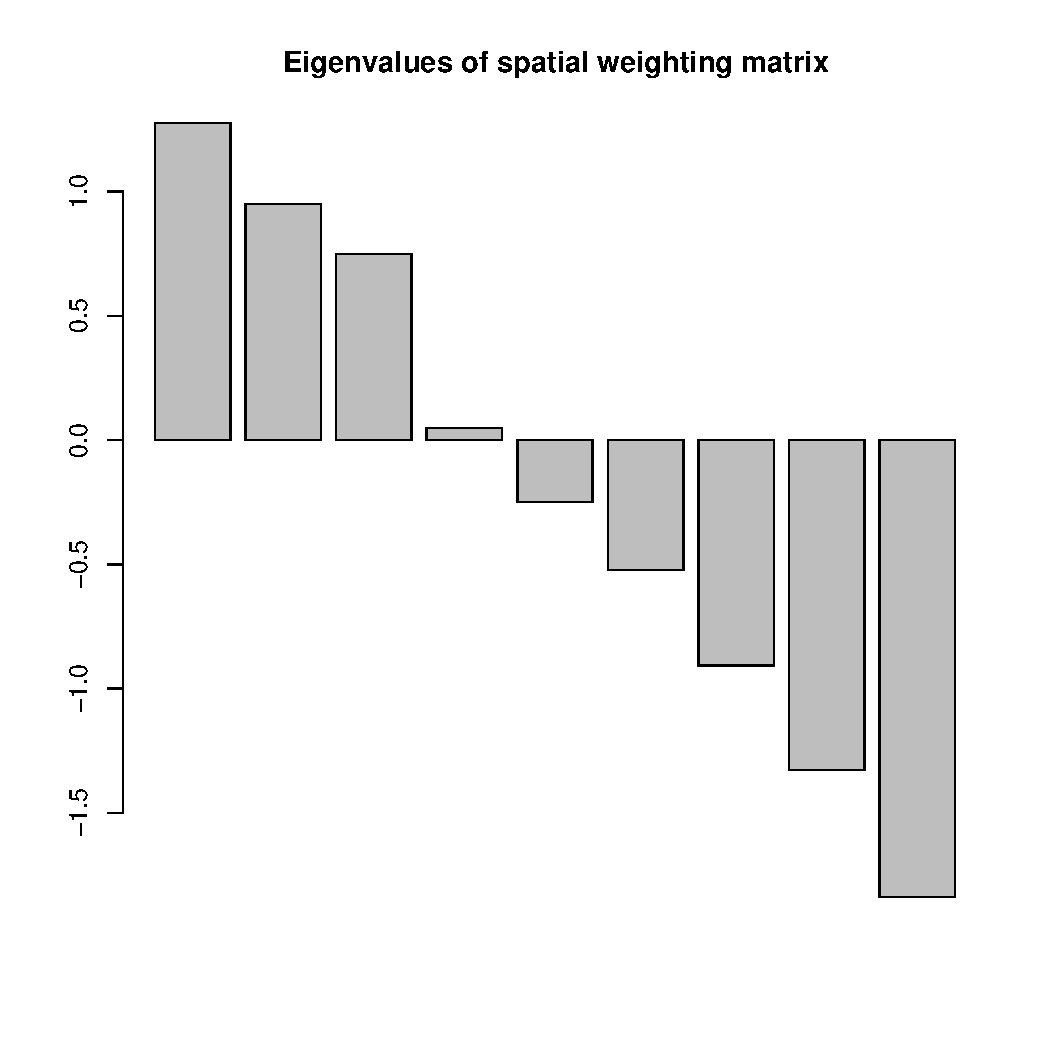
\includegraphics[width=0.8\textwidth,keepaspectratio]{figs/tutorial-ni24}
\end{center}
Eigenvectors can be represented in the geographical space:
\begin{Schunk}
\begin{Sinput}
 par(mfrow = c(3, 3))
 for (i in 1:dim(eigengab$vectors)[2]) s.value(xyir, eigengab$vectors[, 
     i], addaxes = F, sub = paste("Eigenvector", i, "(", 
     round(eigengab$values[i], 3), ")"), cleg = 0, csub = 2, 
     neig = neig(list = nbgab))
\end{Sinput}
\end{Schunk}
\begin{center}
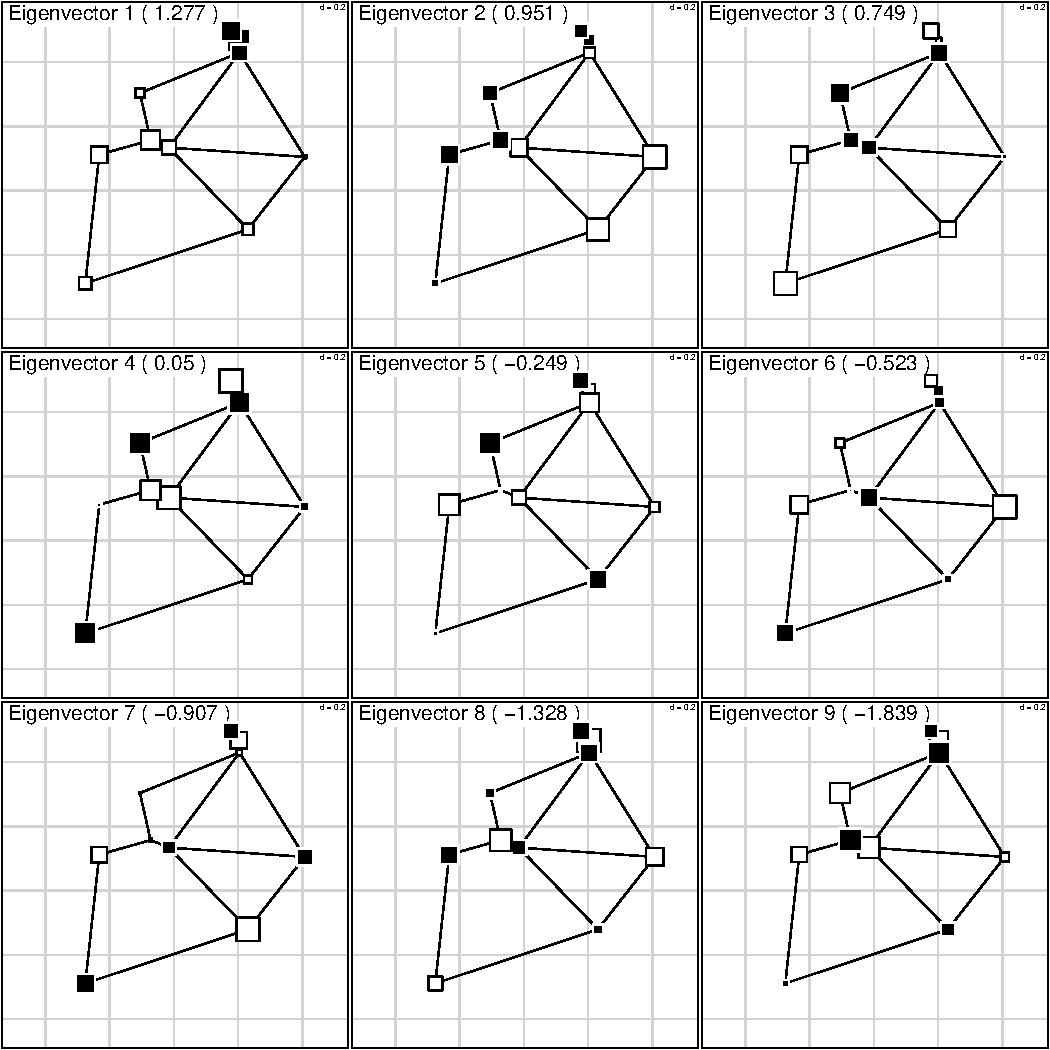
\includegraphics[width=0.8\textwidth,keepaspectratio]{figs/tutorial-ni25}
\end{center}

Moran's I can be computed and tested for each eigenvector with the \texttt{test.scores} function:
\begin{Schunk}
\begin{Sinput}
 moranI <- test.scores(eigengab, listwgab, 99)
 moranI
\end{Sinput}
\begin{Soutput}
      stat pval
1  0.70159 0.01
2  0.52255 0.01
3  0.41162 0.01
4  0.02725 0.28
5 -0.13668 0.56
6 -0.28734 0.28
7 -0.49867 0.07
8 -0.72968 0.01
9 -1.01065 0.01
\end{Soutput}
\end{Schunk}
\begin{Schunk}
\begin{Sinput}
 plot(eigengab$values, moranI$stat, ylab = "Moran's I", 
     xlab = "Eigenvalues", pch = 20, cex = 2)
 text(eigengab$values, moranI$stat, row.names(moranI), 
     pos = 4)
 text(-1, 0.5, paste("correlation =", cor(moranI$stat, 
     eigengab$values)))
 abline(a = 0, b = nrow(xyir)/sum(listw2mat(listwgab)), 
     lty = 3)
\end{Sinput}
\end{Schunk}
\begin{center}
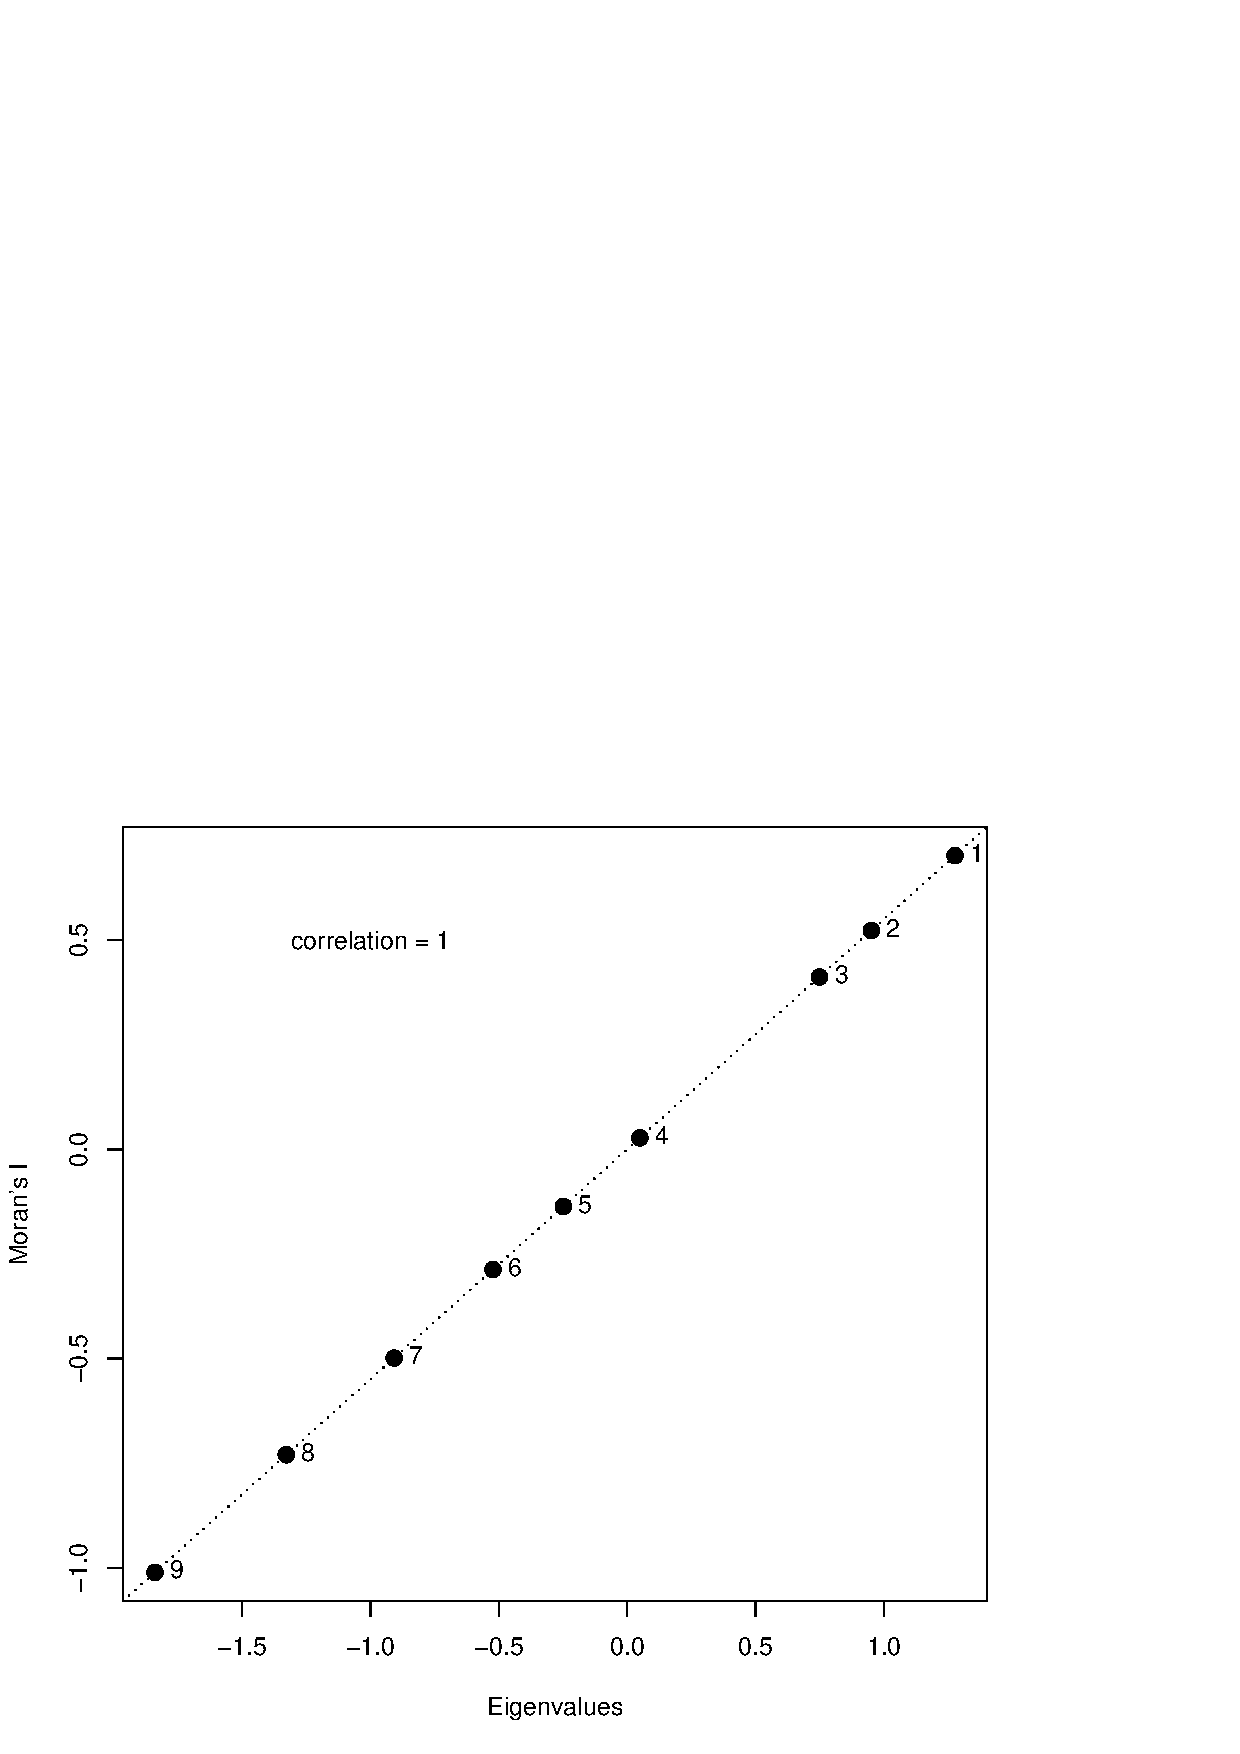
\includegraphics[width=0.8\textwidth,keepaspectratio]{figs/tutorial-ni25c}
\end{center}

Eigenvalues and Moran's I are equal (post-multiply by a constant). Spatial representation of significant eigenvectors:

\begin{Schunk}
\begin{Sinput}
 signi = which(moranI$p < 0.05)
 signi
\end{Sinput}
\begin{Soutput}
[1] 1 2 3 8 9
\end{Soutput}
\begin{Sinput}
 par(mfrow = n2mfrow(length(signi)))
 for (i in signi) s.value(xyir, eigengab$vectors[, i], 
     addaxes = F, sub = paste("ev", i), csub = 2, neig = neig(list = nbgab))
\end{Sinput}
\end{Schunk}
\begin{center}
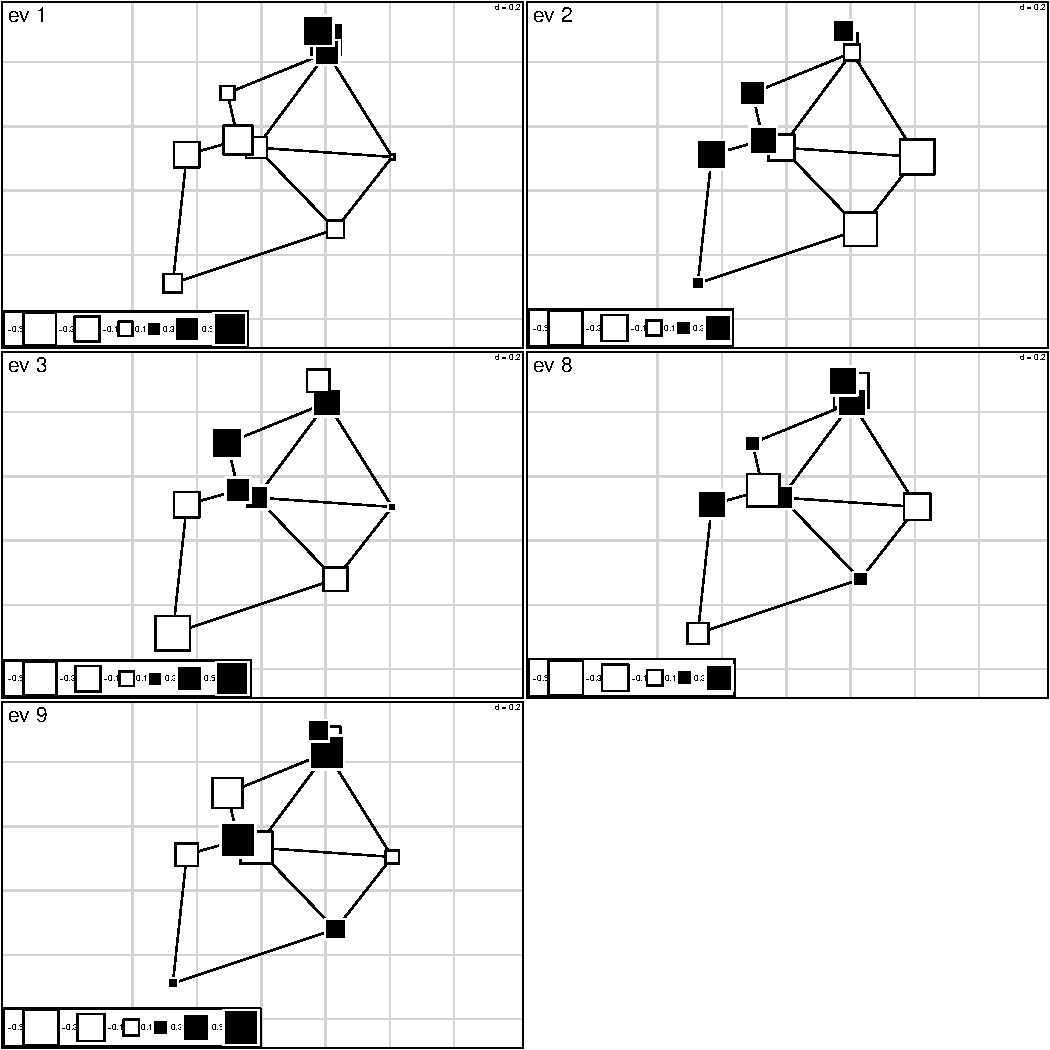
\includegraphics[width=0.8\textwidth,keepaspectratio]{figs/tutorial-ni26}
\end{center}

\section{Selection of a spatial weighting matrix}
The data-driven procedure of selection is based on \textit{AICc}. The function \texttt{ortho.AIC} orders variables and returns \textit{AICc} for all models of one, two, ..., \textit{p}  variables.
We illustrate its use with the oribatid data-set which is available in the \texttt{ade4} package. Data are Hellinger-transformed and then the linear trend is removed:
\begin{Schunk}
\begin{Sinput}
 data(oribatid)
 fau <- sqrt(oribatid$fau/outer(apply(oribatid$fau, 1, 
     sum), rep(1, ncol(oribatid$fau)), "*"))
 faudt <- resid(lm(as.matrix(fau) ~ as.matrix(oribatid$xy)))
\end{Sinput}
\end{Schunk}
For instance, we consider the binary spatial weighting matrix based on the Delaunay triangulation.
\begin{Schunk}
\begin{Sinput}
 nbtri <- tri2nb(as.matrix(oribatid$xy))
 sc.tri <- scores.listw(nb2listw(nbtri, style = "B"))
 AIC.tri <- ortho.AIC(faudt, sc.tri$vec)
 AIC.tri
\end{Sinput}
\begin{Soutput}
 [1]  -90.923  -92.465  -93.783  -94.725  -95.195  -94.967  -94.672
 [8]  -94.306  -93.865  -93.367  -92.620  -91.835  -90.893  -89.893
[15]  -88.797  -87.560  -86.230  -84.784  -83.072  -81.126  -79.055
[22]  -76.853  -74.516  -71.964  -69.248  -66.229  -62.934  -59.436
[29]  -55.708  -51.684  -47.391  -42.795  -37.815  -32.406  -26.587
[36]  -20.286  -13.458   -6.040    2.054   10.816   20.387   30.845
[43]   42.285   54.854   68.671   83.904  100.829  119.706  140.751
[50]  164.349  191.022  221.413  256.372  296.682  343.654  399.072
[57]  465.254  545.311  644.133  769.552  932.074 1150.598 1459.199
[64] 1925.954 2712.519 4298.879 9097.134       NA       NA
\end{Soutput}
\end{Schunk}

The minimum value and the rank of the corresponding are obtained easily:
\begin{Schunk}
\begin{Sinput}
 min(AIC.tri, na.rm = TRUE)
\end{Sinput}
\begin{Soutput}
[1] -95.2
\end{Soutput}
\begin{Sinput}
 which.min(AIC.tri)
\end{Sinput}
\begin{Soutput}
[1] 5
\end{Soutput}
\end{Schunk}

Note that the order of the variables can also be obtained from the function \texttt{ortho.AIC} by setting the \texttt{ord.var} argument to \texttt{TRUE}. In this case, the returned object is a list of two vectors:
\begin{Schunk}
\begin{Sinput}
 AIC.tri <- ortho.AIC(faudt, sc.tri$vec, ord.var = TRUE)
 AIC.tri$AICc[1:10]
\end{Sinput}
\begin{Soutput}
 [1] -90.92 -92.47 -93.78 -94.73 -95.20 -94.97 -94.67 -94.31 -93.86
[10] -93.37
\end{Soutput}
\begin{Sinput}
 AIC.tri$ord[1:10]
\end{Sinput}
\begin{Soutput}
 [1]  3  2  7  1 16  4 10  6 13 57
\end{Soutput}
\end{Schunk}
The user-friendly function \texttt{test.W} simplifies the procedure of selection of a spatial weighting matrix. It takes at least two arguments: a response matrix and an object of the class \texttt{nb}.
If only two arguments are considered, the function prints the results for the best model. All the results are stored in the element \texttt{best} of the list. It contains eigenvectors and eigenvalues of the spatial weighting matrix considered and the results of the \textit{AIC}-based procedure.
\begin{Schunk}
\begin{Sinput}
 tri.res <- test.W(faudt, nbtri)
\end{Sinput}
\begin{Soutput}
Best model:


   AICc NbVar
1 -95.2     5
\end{Soutput}
\begin{Sinput}
 names(tri.res)
\end{Sinput}
\begin{Soutput}
[1] "all"  "best"
\end{Soutput}
\begin{Sinput}
 names(tri.res$best)
\end{Sinput}
\begin{Soutput}
[1] "values"  "vectors" "call"    "AICc"    "AICc0"   "ord"    
[7] "R2"     
\end{Soutput}
\end{Schunk}

The function can also be used to estimate the best values of parameters if we consider a function of the distance.
This can be illustrated with the function $f_2=1-(x^\alpha)/dmax^\alpha$ with the connectivity defined by Delaunay triangulation. We considered the sequence of integers between 2 and 10 for $\alpha$.
\begin{Schunk}
\begin{Sinput}
 f2 <- function(x, dmax, y) {
     1 - (x^y)/(dmax)^y
 }
 maxi <- max(unlist(nbdists(nbtri, as.matrix(oribatid$xy))))
 tri.f2 <- test.W(faudt, nbtri, f = f2, y = 2:10, dmax = maxi, 
     xy = as.matrix(oribatid$xy))
\end{Sinput}
\begin{Soutput}
Best model:


   y dmax   AICc NbVar
9 10    3 -96.22     6
\end{Soutput}
\end{Schunk}
In this case, the element best contains the results for the best values of the parameter $\alpha$ (i.e. $\alpha$=10).
\begin{Schunk}
\begin{Sinput}
 names(tri.f2$best)
\end{Sinput}
\begin{Soutput}
[1] "values"  "vectors" "call"    "AICc"    "AICc0"   "ord"    
[7] "R2"     
\end{Soutput}
\end{Schunk}
Lastly, the function \texttt{test.W} can be used to evaluate different definitions of neighborhood. We illustrate this possibility by the definition of a sequence of neighborhood by distance criteria.
Firstly, we choose the range of values to be tested with an empirical multivariate variogram using the function \texttt{variogmultiv}.
The function has been applied to oribatid mites data:
\begin{Schunk}
\begin{Sinput}
 mvspec <- variogmultiv(faudt, oribatid$xy, nclass = 20)
 mvspec
\end{Sinput}
\begin{Soutput}
$d
 [1] 0.2405 0.7214 1.2023 1.6833 2.1642 2.6452 3.1261 3.6070 4.0880
[10] 4.5689 5.0498 5.5308 6.0117 6.4926 6.9736 7.4545 7.9355 8.4164
[19] 8.8973 9.3783

$var
 [1] 0.2049 0.2326 0.2417 0.2545 0.2829 0.3205 0.3203 0.3361 0.3289
[10] 0.2791 0.2964 0.2709 0.2479 0.2624 0.2371 0.2541 0.2893 0.3343
[19] 0.3752 0.4709

$n.c
 [1] 61 67 70 69 70 70 70 70 70 70 70 66 60 47 43 37 26 18 13  9

$n.w
 [1]  63 135 245 223 272 235 180 189 138 113 134 102 117  65  71  49
[17]  35  25  13  11

$dclass
 [1] "(0,0.481]"     "(0.481,0.962]" "(0.962,1.44]"  "(1.44,1.92]"  
 [5] "(1.92,2.4]"    "(2.4,2.89]"    "(2.89,3.37]"   "(3.37,3.85]"  
 [9] "(3.85,4.33]"   "(4.33,4.81]"   "(4.81,5.29]"   "(5.29,5.77]"  
[13] "(5.77,6.25]"   "(6.25,6.73]"   "(6.73,7.21]"   "(7.21,7.69]"  
[17] "(7.69,8.18]"   "(8.18,8.66]"   "(8.66,9.14]"   "(9.14,9.62]"  
\end{Soutput}
\begin{Sinput}
 plot(mvspec$d, mvspec$var, ty = "b", pch = 20, xlab = "Distance", 
     ylab = "C(distance)")
\end{Sinput}
\end{Schunk}
\begin{center}
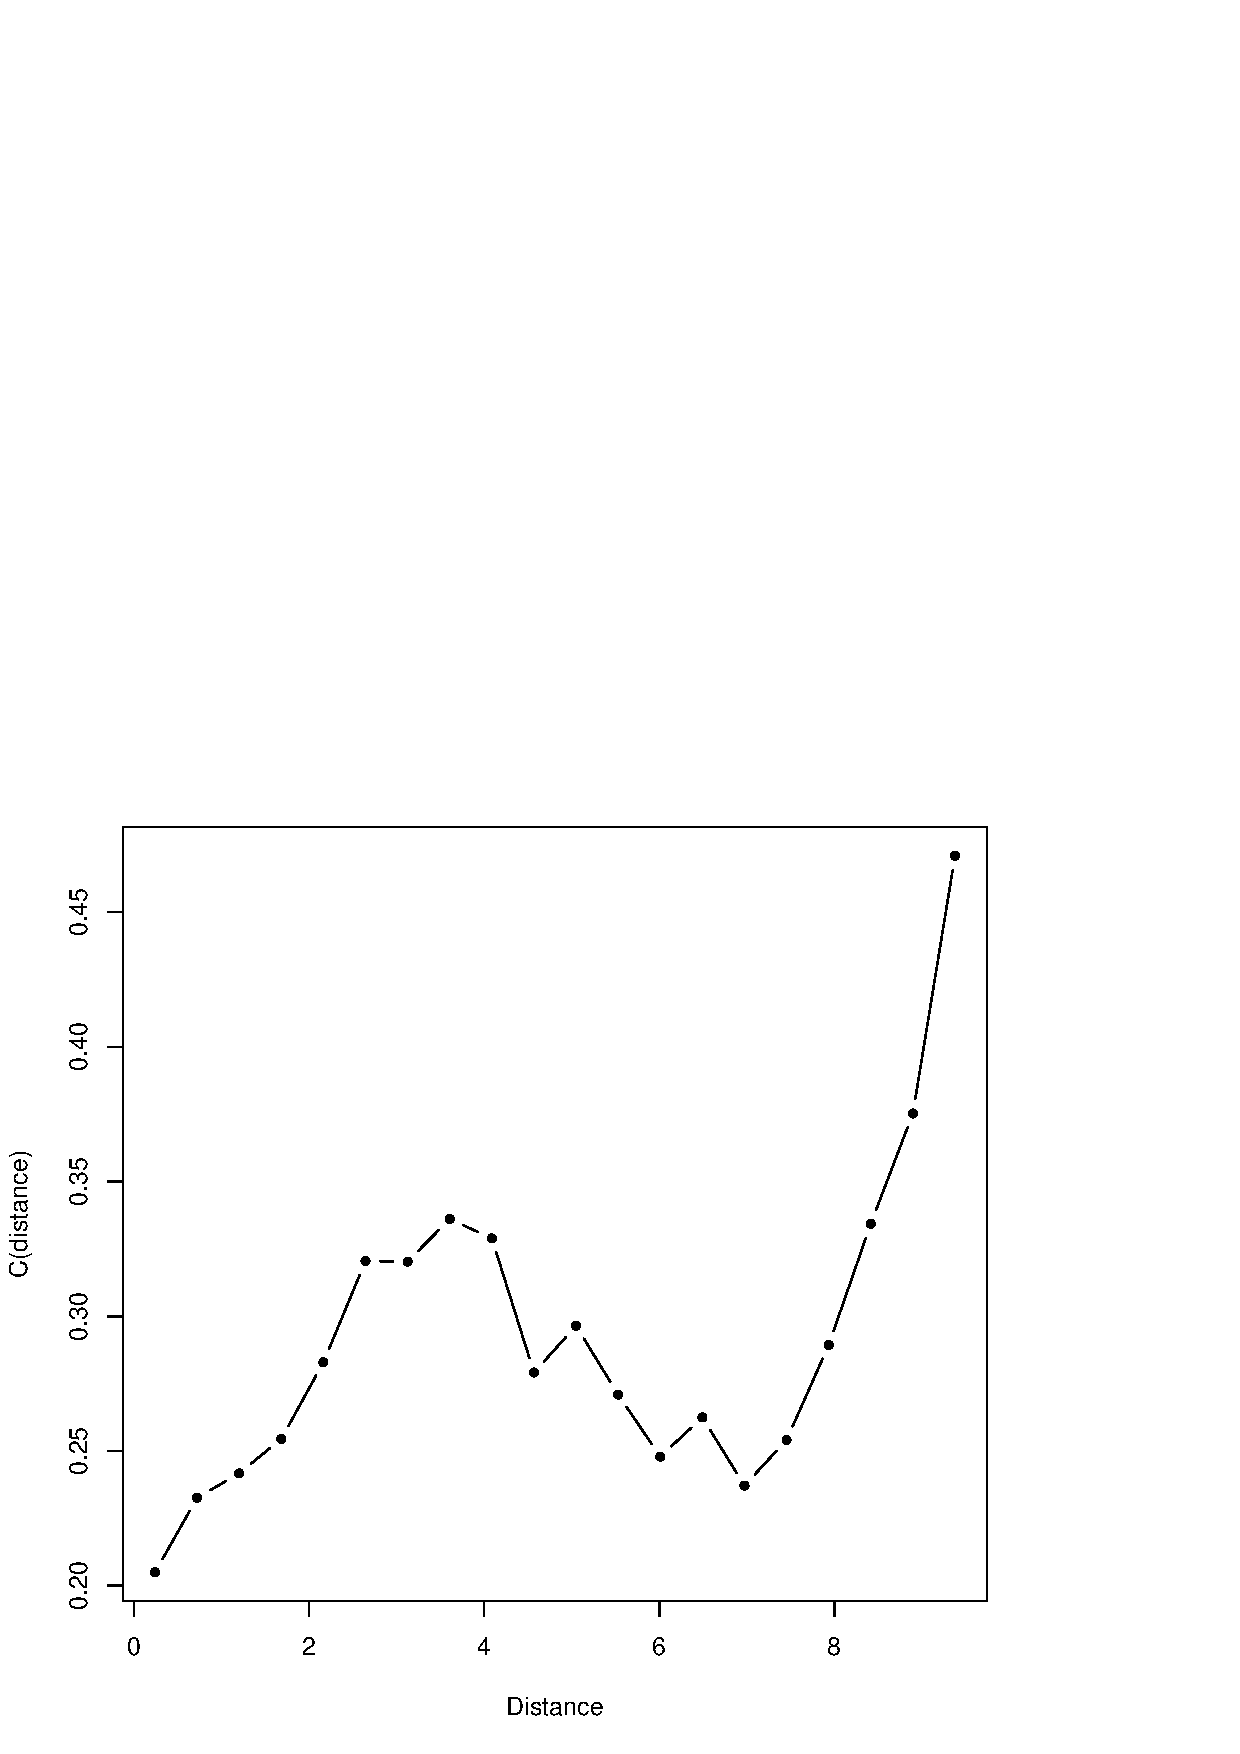
\includegraphics[width=0.8\textwidth,keepaspectratio]{figs/tutorial-ni34}
\end{center}
We will construct ten neighborhood matrices with a distance criterion varying along the sequence of 10 evenly distributed values between 1.012 and 4 m:
\begin{Schunk}
\begin{Sinput}
 dxy <- seq(give.thresh(dist(oribatid$xy)), 4, le = 10)
 nbdnnlist <- lapply(dxy, dnearneigh, x = as.matrix(oribatid$xy), 
     d1 = 0)
\end{Sinput}
\end{Schunk}
Then, the function \texttt{test.W} can be applied to this list of neighborhood matrices:
\begin{Schunk}
\begin{Sinput}
 dnn.bin <- lapply(nbdnnlist, test.W, Y = faudt)
\end{Sinput}
\begin{Soutput}
Best model:


    AICc NbVar
1 -96.65     8


Best model:


    AICc NbVar
1 -97.14     5


Best model:


    AICc NbVar
1 -99.42     7


Best model:


    AICc NbVar
1 -100.6     5


Best model:


    AICc NbVar
1 -99.28     4


Best model:


   AICc NbVar
1 -97.8     5


Best model:


    AICc NbVar
1 -95.23     4


Best model:


    AICc NbVar
1 -96.88     6


Best model:


    AICc NbVar
1 -94.32     6


Best model:


    AICc NbVar
1 -96.72     6
\end{Soutput}
\end{Schunk}
The object \texttt{dnn.bin} is a list with the results of \texttt{test.W} for each neighborhood matrix:
\begin{Schunk}
\begin{Sinput}
 length(dnn.bin)
\end{Sinput}
\begin{Soutput}
[1] 10
\end{Soutput}
\end{Schunk}
For each neighborhood matrix, we can find the lowest \textit{AICc}:
\begin{Schunk}
\begin{Sinput}
 minAIC <- sapply(dnn.bin, function(x) min(x$best$AICc, 
     na.rm = T))
\end{Sinput}
\end{Schunk}
And select the best spatial weighting matrix corresponding to a distance of 2.007 m:
\begin{Schunk}
\begin{Sinput}
 which.min(minAIC)
\end{Sinput}
\begin{Soutput}
[1] 4
\end{Soutput}
\begin{Sinput}
 dxy[which.min(minAIC)]
\end{Sinput}
\begin{Soutput}
[1] 2.007
\end{Soutput}
\end{Schunk}

A similar approach can be used with a spatial weighting function:
\begin{Schunk}
\begin{Sinput}
 f2 <- function(x, dmax, y) {
     1 - (x^y)/(dmax)^y
 }
\end{Sinput}
\end{Schunk}
It is a little bit more complicate if some parameters (here dmax) vary with the neighborhood matrix:
\begin{Schunk}
\begin{Sinput}
 dnn.f2 <- lapply(nbdnnlist, function(x) test.W(x, Y = faudt, 
     f = f2, y = 2:10, dmax = max(unlist(nbdists(x, as.matrix(oribatid$xy)))), 
     xy = as.matrix(oribatid$xy)))
\end{Sinput}
\begin{Soutput}
Best model:


  y  dmax   AICc NbVar
1 2 1.011 -101.1     8


Best model:


  y  dmax   AICc NbVar
3 4 1.342 -98.58     5


Best model:


  y  dmax   AICc NbVar
4 5 1.662 -99.31     9


Best model:


   y  dmax   AICc NbVar
9 10 2.006 -100.4     7


Best model:


  y  dmax   AICc NbVar
1 2 2.332 -102.6     9


Best model:


  y  dmax   AICc NbVar
2 3 2.668 -102.7     7


Best model:


  y dmax   AICc NbVar
1 2    3 -102.5     5


Best model:


  y  dmax   AICc NbVar
1 2 3.329 -100.8     6


Best model:


  y  dmax  AICc NbVar
1 2 3.658 -99.3     3


Best model:


  y dmax  AICc NbVar
1 2    4 -98.6     4
\end{Soutput}
\begin{Sinput}
 minAIC <- sapply(dnn.f2, function(x) min(x$best$AICc, 
     na.rm = T))
 min(minAIC)
\end{Sinput}
\begin{Soutput}
[1] -102.7
\end{Soutput}
\begin{Sinput}
 which.min(minAIC)
\end{Sinput}
\begin{Soutput}
[1] 6
\end{Soutput}
\begin{Sinput}
 dnn.f2[[which.min(minAIC)]]$all
\end{Sinput}
\begin{Soutput}
   y  dmax   AICc NbVar
1  2 2.668 -102.4     7
2  3 2.668 -102.7     7
3  4 2.668 -101.0     5
4  5 2.668 -100.6     5
5  6 2.668 -101.4     6
6  7 2.668 -100.8     5
7  8 2.668 -100.7     6
8  9 2.668 -100.5     5
9 10 2.668 -100.3     5
\end{Soutput}
\end{Schunk}

Lastly, Eigenvectors of the best spatial weighting matrix can be mapped. They are represented by the order given by the selection procedure.
The vector 3 explains the largest part of the oribatid community, then it is the second and the eighth:
\begin{Schunk}
\begin{Sinput}
 par(mfrow = c(1, 3))
 s.value(oribatid$xy, dnn.f2[[7]]$best$vectors[, dnn.f2[[7]]$best$ord[1]], 
     cleg = 0, sub = paste("vector", dnn.f2[[7]]$best$ord[1]), 
     csub = 3)
 s.value(oribatid$xy, dnn.f2[[7]]$best$vectors[, dnn.f2[[7]]$best$ord[2]], 
     cleg = 0, sub = paste("vector", dnn.f2[[7]]$best$ord[2]), 
     csub = 3)
 s.value(oribatid$xy, dnn.f2[[7]]$best$vectors[, dnn.f2[[7]]$best$ord[3]], 
     cleg = 0, sub = paste("vector", dnn.f2[[7]]$best$ord[3]), 
     csub = 3)
\end{Sinput}
\end{Schunk}
\begin{center}
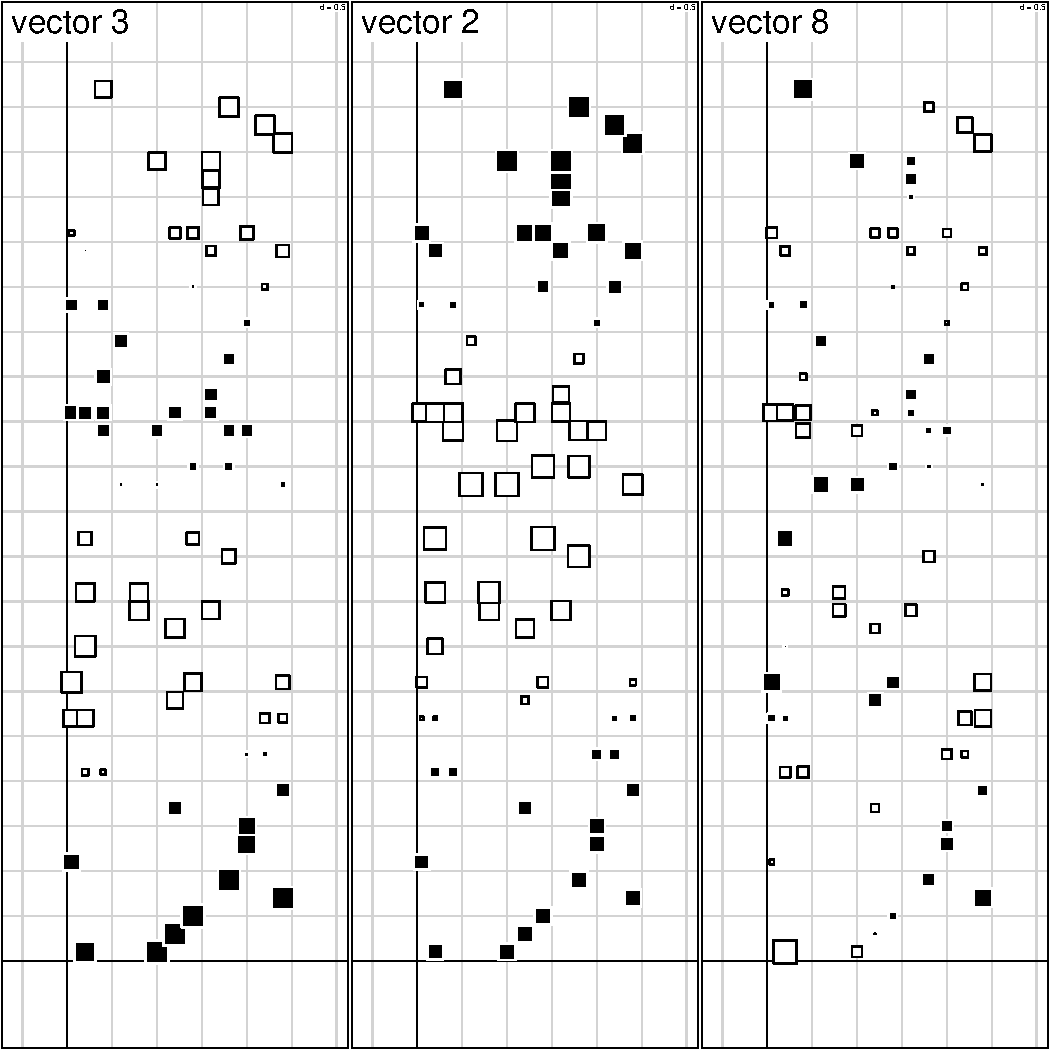
\includegraphics[width=0.8\textwidth,keepaspectratio]{figs/tutorial-ni41}
\end{center}
\end{document}

